\documentclass[
  10pt,
  a4wide,
  double-sided,
  smallheadings
]{article}
\usepackage{a4wide}
\usepackage{microtype} % more pretty letters
\usepackage{graphicx}
\usepackage[absolute]{textpos} % Required to place images, for example the logo 
                               % on the title page
\textblockorigin{0cm}{0cm}
\usepackage{hyperref}
\usepackage[ansinew]{inputenc} % German umlauts
\usepackage[usenames,dvipsnames]{color}
\usepackage{float}
\usepackage{tikz}
\usetikzlibrary{calc,through,backgrounds}
\usepackage{fancyvrb}
\VerbatimFootnotes % Required, otherwise verbatim does not work in footnotes!
\usepackage{listings}
\usepackage{nomencl}
\usepackage{theorem}
\usepackage{pdfpages}

% \makenomenclature

\definecolor{Brown}{cmyk}{0,0.81,1,0.60}
\definecolor{OliveGreen}{cmyk}{0.64,0,0.95,0.40}
\definecolor{CadetBlue}{cmyk}{0.62,0.57,0.23,0}
\definecolor{LightGray}{gray}{0.9}

\newtheorem{algo}{Algorithm}
\newtheorem{prob}{Problem}
\newtheorem{desc}{Description}

% Bold vectors
\renewcommand{\vec}[1]{\mathbf{#1}}

% Lines in the title page
\newcommand{\HRule}{\rule{\linewidth}{0.5mm}}

% PDF related settings
\hypersetup{
  backref,
  colorlinks=false,
  pdfborder=0 0 0,
  pdftitle=Lagrangian Particle Tracking on a GPU.
  pdfauthor=Nils Br\"{u}nggel
}

% Prevent splitting footnotes.
\interfootnotelinepenalty=10000

% Change the title from references to bibliography
\renewcommand\refname{Bibliography}

\begin{document}

% ------------------------------------------------------------------------------
% Listing configuration
\lstset{
    language=C,                             % Code langugage
    basicstyle=\small\ttfamily,             % Code font
    keywordstyle=\color{OliveGreen},        % Keywords font ('*' = uppercase)
    commentstyle=\color{gray},              % Comments font
    numbers=left,                           % Line nums position
    numberstyle=\tiny,                      % Line-numbers fonts
    stepnumber=1,                           % Step between two line-numbers
    numbersep=5pt,                          % How far are line-numbers from code
    backgroundcolor=\color{LightGray},      % Choose background color
    frame=none,                             % A frame around the code
    tabsize=2,                              % Default tab size
    captionpos=b,                           % Caption-position = bottom
    breaklines=true,                        % Automatic line breaking?
    breakatwhitespace=false,                % Automatic breaks only at whitespaces?
    showspaces=false,                       % Dont make spaces visible
    showtabs=false,                         % Dont make tabls visible
    % columns=flexible,                     % Column format BREAKS MONOSPACE!
    morekeywords={                          % C++
        class,
        template,
        public,
        private,
        __global__,
        __device__
    }
}
% ------------------------------------------------------------------------------
    
% TODO logo HSLU

\begin{titlepage}

\begin{textblock*}{8cm}(0cm, -1cm)
    
\includegraphics[width=1\textwidth]{content/gfx/hslu_logo}
\end{textblock*}

\vspace*{4cm}

\begin{center}
    
    \HRule \\[0.4cm]
    { \huge \bfseries Lagrangian Particle Tracking on a GPU}\\[0.4cm]
    \HRule \\[1cm]

    \begin{tabular}{ l c r }
        \emph{Author}            & \hspace*{6cm} & \emph{Advisors} \\
        Nils \textsc{Br\"unggel} & \hspace*{6cm} & Prof. J\"org \textsc{Hofstetter} \\
        & & Prof. Dr. Josef \textsc{B\"urgler}
    \end{tabular}
    \vfill

    {\large \today}

\end{center}

\newpage

\end{titlepage}

\pagenumbering{Roman}       % Roman numbering for the title and the abstract.
\tableofcontents
\newpage
\listoffigures
\newpage

\thispagestyle{empty}
\section*{Erkl\"arung der Selbstst\"andigkeit}
\thispagestyle{empty}

Hiermit erkl\"are ich, dass ich die vorliegende Arbeit selbstst\"andig angefertigt und keine anderen als die angegebenen Hilfsmittel verwendet habe. S\"amtliche verwendeten Textausschnitte, Zitate oder Inhalte anderer Verfasser wurden ausdr\"ucklich als solche gekennzeichnet.
\vspace{4\baselineskip}\\
Horw, 15. Juli 2011 \hfill Nils Br\"unggel
\vspace{4\baselineskip}\\
%\clearpage
%\mbox{}\thispagestyle{empty}
\section*{Acknowledgments}

I would like to thank the many people who helped me completing this thesis. Especially my advisor Josef B\"urgler who took the time to discuss the many problems I ran into during this work and helped me to develop solutions for it. Brahim Aakti who thought me many things about fluid dynamics that I never learned as a computer science student. Thomas Koller who helped me better understanding C++ and reviewed my software design. Luca Mangani for discussing the implementation in OpenFOAM. And all the people who read this thesis (or parts of it) and gave feedback: Antoine Hauck, Kym Br\"unggel, Marcel Br\"unggel and David Roos Launchbury.

% \begin{abstract}
% Complex fluid dynamic simulations often require the tracking of particles. For example when simulating sprays for direct fuel injection into a combustion engine or for a simulation coupling the probability density function (PDF) method with the finite volume method (FVM). A practical fluid simulation needs to handle arbitrary geometries imported from a computer aided design (CAD) system. Therefore unstructured mesh handling is required. In an unstructured mesh particle-tracking is non-trivial and requires a sophisticated algorithm. Based on an existing algorithm an efficient particle tracking engine for large number of particles was developed. In order to speed up the algorithms, a graphics processing unit (GPU) was used which can process thousands of particles in parallel. Compared to the single threaded implementation in OpenFOAM, an open source computational fluid dynamics software, the newly-developed parallel implementation is around 30 times faster.
% \end{abstract}

%\section{*Summary}
\begin{abstract}
    
% Ausganslage
In addition to the most common numerical method, the finite volume method, particles are often used in complex fluid simulations. For example when simulating combustion in a Diesel engine the droplets are modeled as particles while the fluid is calculated in a discrete mesh. The two phases are called Eulerian and Lagrangian. While the Lagrangian phase does not need a mesh itself, coupling it with the Eulerian phase requires to know, for each time step, in which cell the particles reside. If unstructured meshes are used it is not trivial to find a particles occupancy cell, given its position. To do so a sophisticated particle tracking algorithm was developed.

% Ziel
When using particles it is usually desirable to use a large number of particles, because this leads to better results. The aim of this project was to track particles more efficiently. Because the particle tracking algorithm tracks each particle individually it is suitable for massively parallel computing. A graphics processing unit (GPU) was used which can run thousands of threads concurrently.

% Weg
Using an existing computational fluid dynamics (CFD) package, OpenFOAM, a simple solver was developed in which particles are dragged by a given velocity field through the mesh. This work involved converting the mesh and particle data into structures suitable for parallel processing as well as porting the algorithm to the GPU. Testing and validating the code was the biggest part: Because of the lack of object oriented constructs for the code on the GPU, the data was stored in simple arrays making it necessary to calculate array indices in the program. This lead to rather error prone code. To ensure correctness the intermediate results of the sequential implementation were extracted and compared to the results of the new parallel implementation. Finally a switch was added to the solver which causes a mesh search after each time-step: For each particle a mesh search is executed for its end position revealing the actual occupancy cell. This is then compared with the new occupancy calculated by the newly-developed  particle tracking algorithm.  If it is turned on, one can ensure that occupancy cells of all particles are correct. This, of course, makes the solver extremely slow.

% Ergebnise
Comparing the computation time for the tracking algorithm revealed a huge speedup. The GPU implementation is around 30 times faster compared to the sequential implementation in OpenFOAM. Because it is necessary to copy all the data over a slow bus to the GPU the practical execution time is slower, but still much faster than the sequential implementation.

\end{abstract}

% \printnomenclature

\pagenumbering{arabic}      % Arabic numbering later

% % Put this into abstract for the final version

\section*{Summary}

% Ausganslage
In addition to the most common numerical method, the finite volume method, particles are often used in complex fluid simulations. For example when simulating combustion in a Diesel engine the droplets are modeled as particles while the fluid is calculated in a discrete mesh. The two phases are called Eulerian and Lagrangian. While the Lagrangian phase does not need a mesh itself, coupling it with the Eulerian phase requires to know, for each time step, in which cell the particles reside. If unstructured meshes are used it is not trivial to find a particles occupancy cell, given its position. To do so a sophisticated particle tracking algorithm was developed.

% Ziel
When using particles it is usually desirable to use a large number of particles, because this leads to better results. The aim of this project was to track particles more efficiently. Because the particle tracking algorithm tracks each particle individually it is suitable for massively parallel computing. A graphics processing unit (GPU) was used which can run thousands of threads concurrently.

% Weg
Using an existing computational fluid dynamics (CFD) package, OpenFOAM, a simple solver was developed in which particles are dragged by a given velocity field through the mesh. This work involved converting the mesh and particle data into structures suitable for parallel processing as well as porting the algorithm to the GPU. Testing and validating the code was the biggest part: Because of the lack of object oriented constructs for the code on the GPU, the data was stored in simple arrays making it necessary to calculate array indices in the program. This lead to rather error prone code. To ensure correctness the intermediate results of the sequential implementation were extracted and compared to the results of the new parallel implementation. Finally a switch was added to the solver which causes a mesh search after each time-step: For each particle a mesh search is executed for its end position revealing the actual occupancy cell. This is then compared with the new occupancy calculated by the newly-developed  particle tracking algorithm.  If it is turned on, one can ensure that occupancy cells of all particles are correct. This, of course, makes the solver extremely slow.

% Ergebnise
Comparing the computation time for the tracking algorithm revealed a huge speedup. The GPU implementation is around 30 times faster compared to the sequential implementation in OpenFOAM. Because it is necessary to copy all the data over a slow bus to the GPU the practical execution time is slower, but still much faster than the sequential implementation.
\section{Introduction}

\subsection{Motivation}

In computational fluid dynamics (CFD) the finite volume method (FVM) is most commonly used to solve the partial differential equations (PDE) which describe the fluid flow. In order to discretize the simulation domain a mesh is constructed which covers the whole domain. The equations are then evaluated at the centroid of each cell and the results, such as velocity, pressure, temperature, etc are stored for each cell. In addition to the FVM some parts of a simulation may be modeled as particles such as Diesel droplets in an engine. \cite{nordin00} The gaseous phase, represented in the mesh, is called \emph{Eulerian}, while the liquid phase, represented by particles, is called \emph{Lagrangian}. Those are different ways of looking at the flow field. In the Lagrangian view the observer follows an individual particle as it moves through space and time. This can be visualized as sitting in a boat and drifting down a river. The Eulerian specification of the flow field is a way of looking at fluid motion that focuses on specific locations in space through which the fluid flows as time passes. This can be visualized by sitting on the bank of a river and watching the water pass the fixed location. \cite{eulerianLagrangian} There are different levels of coupling between these two phases: If the Lagrangian particles are just dragged by the Eulerian phase one refers to this as a \emph{one-way coupling}. If the Lagrangian particles also influence the Eulerian phase it is called a \emph{two-way coupling}. The mesh plays an important role when the two phases are coupled: The Eulerian equations are evaluated at the centroid of every cell. The Lagrangian particles do not need a mesh themselves, but the coupling requires it to know in which cell a particle resides so that the coupling terms can be appended to the Eulerian phase. \emph{More specifically we need to know for every time step through which cells the particle travels and how much time it spends in each cell.}

It is distinguished between structured and unstructured meshes. Structured refers to the way how the mesh data is stored in memory: A direct mapping between the connections in the mesh and the addresses of the data exists. This structure restricts the shape of the cells in the mesh to hexahedra. Unstructured meshes on the other hand allow cells with any number of faces, this makes them more flexible but also increases the amount of work a program has to do, for example to access a cell next to a given cell. Structured meshes can be transformed into a uniform cartesian grid. \cite{innovativeCFDGrid} It is therefore trivial to find the cell in which a particle resides, given its position. In an unstructured mesh this is no longer possible and requires a sophisticated algorithm which is explained in section \ref{sec:particleTrackingAlgo}. OpenFOAM comes with support for unstructured meshes because this makes it simpler to automatically mesh complex geometries from a CAD system and it simplifies the import of meshes from different meshing tools. \cite{jasakMeshHandling}

\subsection{Project Goal}

Particle tracking requires the execution of simple vector calculations for a large number of particles. This can be achieved more efficiently by using a massively parallel processor such as a GPU (see section \ref{sec:gpuComputing}).
Based on the existing OpenFOAM code the goal is to develop a solver which moves particles using the velocity field from the mesh. The solver will use the GPU to execute the computations required for the particle tracking algorithm in a massively parallel way, which will lead to great speedup compared to the already existing single-threaded implementation in OpenFOAM. The original project definition can be found in the appendix, section \ref{sec:projectDef}.

\section{OpenFOAM}
\label{sec:OpenFOAM}

\subsection{Introduction}

OpenFOAM is an open source framework for computational fluid dynamics. It is entirely written in C++ and licensed under the GNU General Public License (GPL). OpenFOAM comes with basic meshing tools, various solvers and utilities to import meshes and export data for post processing. As opposed to many commercial packages the OpenFoam tools do not provide a graphical user interface. Instead the user has to edit configuration files within an OpenFOAM case and then run the solver in a UNIX-like fashion on the command line. One of the strengths of OpenFOAM is that custom solvers can be written or modified quickly because of its modular design and the usage of advanced C++ features.

\subsection{Mesh Representation}
\label{sec:meshRepresentation}

OpenFOAM supports unstructured polyhedral meshes with any number of faces. The mesh is described in the official Users Guide \cite{ug08} (chapter 5), the Programmers Guide \cite{pg08} (chapter 2.3) as well as in Jasak's PhD thesis \cite{jasak96} (chapter 3.2). Here I will recall a short summary. OpenFOAM stores the mesh in the following files\footnote{Located in \verb+constant/polyMesh+ in an OpenFoam case directory.}, which are generated by mesh utilities such as \verb+blockMesh+.

\begin{itemize}

	\item \verb+points+ Contains a list of coordinates of vertices. OpenFOAM implicitly indexes the points starting from 0 up to the number of points minus one.

	\item \verb+faces+ Contains a list of faces. The point indices defined in the \verb+points+ file are used to reference the vertices. It is distinguished between internal faces and boundary faces: Internal faces are between two cells and always have an owner and a neighbour cell assigned, while boundary faces lie on the boundary of the computational domain and just have an owner cell assigned (see below). Further a face normal is defined, so that it points outside of the owner cell. In case the face is a boundary face, the normal points outside of the computational domain.

The order of the vertices of a face is defined such that, if the normal vector points towards the viewer, the vertices are arranged in an anti-clockwise path. The faces are also implicitly indexed, starting with 0 for the first face.

It is common that the faces inside the simulation domain, called inner faces have a lower face label than those on the boundary, called boundary faces. OpenFOAM lets the user define various boundary conditions by referring a set of boundary faces.

	\item \verb+owner+ Each face is assigned an owner cell, in case of an internal face this is the cell with the lower label of the two cells adjacent to the face. The face normal can also be defined as pointing from the cell with the lower label to the cell with the higher label.

	\item \verb+neighbour+ Internal faces also have a neighbour cell. Since an internal face is always between two cells, the cell not being the owner is the neighbour cell. (Which is the cell with the higher label.) Faces lying on the boundary have no neighbour cell and are omitted in the neighbour list. Since some faces always lie on the boundary, this list has less items then the owner list.

	\item \verb+boundary+ The boundary file contains a list of patches which refer to a set of boundary faces.
	
\end{itemize}

\subsection{The Lagrangian Framework}
\label{sec:lagrangianFramework}

OpenFOAM includes a Lagrangian framework which was originally developed to simulate Diesel droplets \cite{nordin00}. The simplest Lagrangian library allows the simulation of solid particles which are moved by the Eulerian field. The work carried out here is based on the \verb+solidPartilce+ library.

\begin{figure}[H]
  \centering
  \includegraphics[scale=0.6]{content/gfx/solidParticleClasses.pdf}
  \caption{Class diagram outlining the solidParticle library.}
  \label{gfx:solidParticleClasses}
\end{figure}

Figure \ref{gfx:solidParticleClasses} shows the most important classes belonging to the solidParticle library. Note that, for the sake of simplicity not all class members are shown. The particles are stored in a doubly linked list. The particle tracking algorithm is implemented in a flexible way: The most basic functionality is in the \verb+Particle+ class via the \verb+trackToFace()+ function. Functionality specific to a certain particle type, such as the drag model, is implemented in the \verb+solidParticle+ class. The \verb+solidParticle+ class provides the \verb+move()+ method which is called from the \verb+solidParticleCloud+ class for every particle. Using the specific drag model the destination for a particle is estimated, \verb+trackToFace()+ is then called with the before calculated destination.

\paragraph{Usage of curiously recurring template patterns}

When looking at the classes of the \verb+solidParticle+ library a remarkable circular dependency between derived classes can be found. For example the classes \verb+Particle+ and \verb+solidParticle+ in the Lagrangian framework. \verb+solidParticle+ is derived from the \verb+Particle+ class template which takes the type of the derived class as template argument.

\begin{figure}[H]
  \centering
  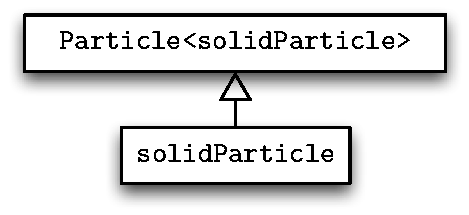
\includegraphics[scale=0.6]{content/gfx/solidParticle.pdf}
  \caption{Illustration of circular dependencies in OpenFOAM using templates and inheritance.}
  \label{gfx:solidParticle}
\end{figure}

% TODO Why exactly is this allowed? By the standard templates are instantiated 
% first and then?

The dependency goes in one direction via inheritance and in the other direction via templates. This pattern was named ''Curiously Recurring Template Pattern (CRTP)'' by James Coplien in 1995 \cite{coplien95}. It can be used to implement static polymorphism without the need to use virtual functions, as illustrated in the example below.

\begin{lstlisting}
#include <cstdio>

template <class DerivedType>
struct A {

    void doSomething() {
        static_cast<DerivedType&>(*this).doSomethingElse();
    }
};

struct B: public A<B> {

    void doSomethingElse() {
        
        printf("Hello from B!\n");
    }
};

struct C: public A<C> {
    
    void doSomethingElse() {
        
        printf("Hello from C!\n");
    }
};


int main() {
    
    B b;
    b.doSomething();
    C c;
    c.doSomething();
    
    return 0;
}

// Output

Hello from B!
Hello from C!

\end{lstlisting}

As mentioned before this idiom is used in the Lagrangian classes\footnote{This can be found in the OpenFOAM source tree in the directory \verb+src/lagrangian+}. The \verb+Particle+ class is declared as follows:

\begin{lstlisting}
template<class ParticleType>
class Particle : public IDLList<ParticleType>::link {
    //..
};
\end{lstlisting}

And the \verb+solidParticle+ class as follows:

\begin{lstlisting}
class solidParticle : public Particle<solidParticle> {
    //..
};
\end{lstlisting}

The particle class can now call members which are to be defined in their derived classes using a static cast on the \verb+this+-pointer.

\begin{lstlisting}
static_cast<ParticleType&>(*this)
\end{lstlisting}

Using a reference to the derived type it can be checked weather the particle is of a special type as done on line 299 from the file \verb+Particle.C+:

\begin{lstlisting}
//..
else if (static_cast<ParticleType&>(*this).softImpact())
{

//..
\end{lstlisting}

This is just one example in which this idiom is used and there are many more within the code of OpenFOAM.

\subsection{Parallelization and Support for GPUs}

The OpenFOAM code is mostly sequential C++ code. Larger simulations can be decomposed into various domains and multiple instances of a solver can be launched which communicate using the message passing interface (MPI) \cite{openfoamParallel}. While OpenFOAM currently does not support fine grained parallelism, it has recently been shown that OpenFOAM could benefit a hybrid parallelization model where OpenMP is used in addition to MPI for the fine grained parallelization on each host \cite{liu11}.

There is officially no support for GPU computing in OpenFOAM, however various third-party solutions exist. The \cite{speedit} SpeedIT tools make it possible to use OpenFOAM with CUBLAS, Nvidia's implementation of BLAS (Basic Linear Algebra Subprograms). OFGPU \cite{ofgpu} runs the Preconditioned conjugate gradient solver for symmetric matrices (PCG) and the Preconditioned biconjugate gradient solver for asymmetric matrices (PBiCG) on the GPU by using the CUSP \cite{cusp} library, a library for sparse linear algebra and graph computations on the GPU.
\section{The Particle Tracking Algorithm}
\label{sec:particleTrackingAlgo}

The particle tracking algorithm used in OpenFOAM was published in \cite{macpherson08}. Since it is crucial for the optimization it is presented here.

\subsection{Basic Particle Tracking Algorithm}

\begin{figure}[H]
  \centering
  \begin{tikzpicture}

% Coords of the Axes
\coordinate (Zero)  at (0,0);
%\coordinate [label=below:$x$](Xend)  at (10,0);
%\coordinate [label=right:$y$](Yend)  at (0,10);

% Coords for cell A
\coordinate (f1start) at (0.5,2);
\coordinate (f1end) at (12,3);
\coordinate (f2start) at (10,1);
\coordinate (f2end) at (11,8);
\coordinate (f3start) at (12,7);
\coordinate (f3end) at (1,8);
\coordinate (f4start) at (3,9);
\coordinate (f4end) at (1,1);

% Intersection between the cell faces: k, l, m, n
% Syntax note: Do NOT make a space between the coord and the --!
% Bottom left
\coordinate (k) at (intersection of f1start--f1end and f4start--f4end);
% Bottom right
\coordinate [label={below right:cell b}] 
	(l) at (intersection of f1start--f1end and f2start--f2end);
% Top right
\coordinate [label={below left:cell a},label={below right:cell c}]  
	(m) at (intersection of f2start--f2end and f3start--f3end);
% Top left
\coordinate (n) at (intersection of f3start--f3end and f4start--f4end);

% Add the face indexes, note that only coordinates and nodes can have labels
\coordinate [label=below:$0$] (0) at ($ (k)!.5!(l) $);
\fill[black] (0) circle (2pt);
\coordinate [label=left:$1$, label={below right:$\mathbf{C_f}$}] 
	(1) at ($ (l)!.5!(m) $);
\fill[black] (1) circle (2pt);
\coordinate [label=above:$2$] (2) at ($ (m)!.5!(n) $);
\fill[black] (2) circle (2pt);
\coordinate [label=left:$3$] (3) at ($ (n)!.5!(k) $);
\fill[black] (3) circle (2pt);

% Centroid
\coordinate (sum) at  ($ (k)+(l)+(m)+(n) $);
\coordinate [label=left:$\mathbf{C_c}$] (Cc) at ($ 1/4*(sum) $);
\fill[black] (Cc) circle (2pt);

% Draw the lines, which define cell A, B and C
%\draw [thin,->] (Zero) -- (Xend);
%\draw [thin,->] (Zero) -- (Yend);
\draw (f1start) -- (f1end);
\draw (f2start) -- (f2end);
\draw (f3start) -- (f3end);
\draw (f4start) -- (f4end);

% Cf
\coordinate[label=right:$\vec{S_f}$] (S) at ($(1)!0.5! -90:(m)$);
\draw [->,dashed] (1) -- (S);

% Particle movement
\coordinate[label=right:$\textbf{a}$] (a) at (8,6);
\coordinate[label=right:$\textbf{b}$] (b) at (12,2);

\coordinate[label=right:$\textbf{p}$] (p) at 
	(intersection of a--b and f2start--f2end);
\coordinate[label=above:$\textbf{p'}$] (p_) at 
	(intersection of a--b and f1start--f1end);

\draw[fill=white,thick,->] (a) -- (b);

\draw[fill=white,dashed,->] (Cc) -- (b);

\filldraw[fill=white] (a) circle (2pt);
\filldraw[fill=white] (p) circle (2pt);
\filldraw[fill=white] (p_)circle (2pt);
\filldraw[fill=white] (b) circle (2pt);

\end{tikzpicture}
  \caption{Example situation in two dimensions illustrates the particle tracking algorithm.}
  \label{fig:f2f}
\end{figure}

For the Lagrangian-Eulerian coupling it is required to know, for every time step, which cells a particle crosses and how much time it spent there. Figure \ref{fig:f2f} illustrates the particle tracking algorithm during a time step. The particle is initially located at position $\vec{a}$ and moves to $\vec{b}$. While traveling along the straight line from $\vec{a}$ to $\vec{b}$ it changes the cell twice at $\vec{p}$ and $\vec{p'}$.

The point where the particle hits the face is calculated by the following equation:

\begin{equation}
  \label{eq:1}
  \vec{p} = \vec{a} + \lambda_a \cdot (\vec{b}-\vec{a})
\end{equation}

$\lambda_a$ denotes the fraction of the path vector which the particle travels until it hits the first face (the distance from $\vec{a}$ to $\vec{p}$). In this equation $\lambda_a$ and $\vec{p}$ are unknown, we only know the start and end position of the particle ($\vec{a}$ and $\vec{b}$). The vector from $\vec{C_f}$ to $\vec{p}$ along the face is orthogonal to the face normal. This leads to the definition of another equation, which can be used to calculate $\vec{p}$:

\begin{equation}
 \label{eq:2}
 (\vec{p} - \vec{C_f}) \bullet \vec{S_f} = 0
\end{equation}

In the equation above we used the fact that the dot product of two orthogonal vectors is zero. Now substituting equation (\ref{eq:1}) into equation (\ref{eq:2}) and solving for $\lambda_a$ gives:

\begin{equation}
  \label{eq:3}
  \lambda_{a} = \frac{(\vec{C_f} - \vec{a}) \bullet \vec{S_f}}
                       {(\vec{b} - \vec{a}) \bullet \vec{S_f}}
\end{equation}

Now since $\vec{p}$ no longer appears in equation (\ref{eq:3}) we can calculate $\lambda_{a}$ for each face respective of the cell. The face with the smallest $\lambda_{a} \in [0, 1]$ is the face, which is crossed by the particle. The particle is then moved along the line from $\vec{a}$ to $\vec{b}$ onto the face hit i.e. $\vec{p} = \vec{a} + \lambda_a \cdot (\vec{b} - \vec{a})$. The particles's occupancy information is updated to the cell on the other side of the face. The next tracking event works in the same way as the one just presented. This is repeated until the whole time step is processed. If $\lambda_{a}$ is not in the interval $[0,1]$, then the particle's end position $\vec{b}$ must be inside the same cell.

\subsection{Modified Tracking Algorithm}

If a face is defined by more than three vertices, then these do not necessarily lie in a plane. In case a face is non-planar the mesh stores the face centroid and interpolates a normal vector which represents the effective plane of the face. When using the effective planes as cell faces, the cells in a mesh are no longer space-filling! It is therefore possible to loose track of a particle when it crosses a face close to a vertex. The deficiencies of the basic particle tracking algorithm are further described in \cite[page 267]{macpherson08}.  While these deficiencies seem to appear in rather large non-standard cases it should be mentioned that the modified tracking algorithm also solves a simple implementation problem of the basic particle algorithm: Just naively moving the particle onto the face hit and then evaluate the formula for $\lambda_a$ again for the new occupancy cell may yields the same face again as before, depending on how the dices of floating point accuracy roll. The problem can be solved by moving the particle just a little bit more into the next cell using an $\epsilon$-environment or by disabling the face in the subsequent calculation\footnote{In the authors experience the first solution, using an $\epsilon$-environment did not work in all cases, it was necessary to disable the face hit for the next calculation.}. There is no such problem when using the modified tracking algorithm, since the cell centre is taken as reference point inside the cell and not the particles actual position in order to get a list of faces which might be hit by the particle.

With reference to figure \ref{fig:f2f}, instead of taking the starting point of a particle, the cell centre is taken as reference point inside the cell to determine which faces the particle may crosses (if any). Replacing $\vec{a}$ with $\vec{C_c}$ in equation (\ref{eq:3}) gives:

\begin{equation}
  \label{eq:4}
  \lambda_{c} = \frac{(\vec{C_f} - \vec{C_c}) \bullet \vec{S_f}} 
                       {(\vec{b} - \vec{C_c}) \bullet \vec{S_f}}
\end{equation}

The line from $\vec{C_c}$ to $\vec{b}$ (shown dashed in figure \ref{fig:f2f}) crosses face 1 and 0\footnote{Or more precisely the plane which is defined by the face normal of face 0.}. Equation (\ref{eq:4}) therefore yields $\lambda_{c}$ between 0 and 1 for face 0 and face 1. If there is no face with  $\lambda_{c} \in [0,1]$, then $\vec{b}$ must be in the same cell as $\vec{a}$. Otherwise it is also necessary to calculate $\lambda_{a}$ using equation (\ref{eq:3}) for the faces, which are crossed by the line from $\vec{C_c}$ to $\vec{b}$ (face 0 and 1 in this case). The lowest value of $\lambda_{a}$ determines then which face was actually hit and the fraction of the time step, which it took to travel to the face can be determined using $\lambda_{a}$. The cell occupancy is changed to the neighbouring cell of the face which was crossed (c in this case). With $\lambda_m = min(1,max(0,\lambda_{a}))$ equation (\ref{eq:moveParticleModified}) is then used to move the particle to p.

\begin{equation}
	\label{eq:moveParticleModified}
	\vec{p} = \vec{a} + \lambda_m \cdot ( \vec{b} - \vec{a} )
\end{equation} 

The complete tracking algorithm is shown below as pseudo code. This was taken from \cite{macpherson08} (algorithm 1).

\begin{algo}{Complete tracking algorithm}
\label{alg:ttf}

	\textbf{while} the particle has not yet reached its end position at $\vec{b}$ \textbf{do}
	
	\noindent\hspace*{1cm}find the set of faces, $F_i$ for which $0 \leq \lambda_c \leq 1$
	
	\noindent\hspace*{1cm}\textbf{if} size of $F_i=0$ \textbf{then}
	
	\noindent\hspace*{2cm}move the particle to the end position
	
	\noindent\hspace*{1cm}\textbf{else}
	
	\noindent\hspace*{2cm}find face $f \in F_i$ for which $\lambda_a$ is smallest
	
	\noindent\hspace*{2cm}move the particle according to equation \ref{eq:moveParticleModified} using this value of $\lambda_a$.
	
	\noindent\hspace*{2cm}set particle cell occupancy to neighbouring cell of face $f$
	
	\noindent\hspace*{1cm}\textbf{end if}

\textbf{end while}

\end{algo}

\subsection{Implementation in OpenFOAM (solidParticle Library)}

The actual implementation of the particle tracking algorithm is more complicated. In the example presented to explain the particle tracking algorithm (figure \ref{fig:f2f}) the velocity of the particle was assumed to be constant during the whole tracking step. In the \verb+solidParticle+ library the velocity of the particle is coupled to the velocity of the fluid: A drag model is used, which calculates the drag issued by the fluid phase onto the particle, assuming spherical particles. In other words the velocity of the particle depends on the velocity of the cell in which it resides and therefore the velocity changes once the particle changes the cell. Therefore, it is required to distinguish between Eulerian and Lagrangian time steps.

\begin{figure}[H]
  \centering
  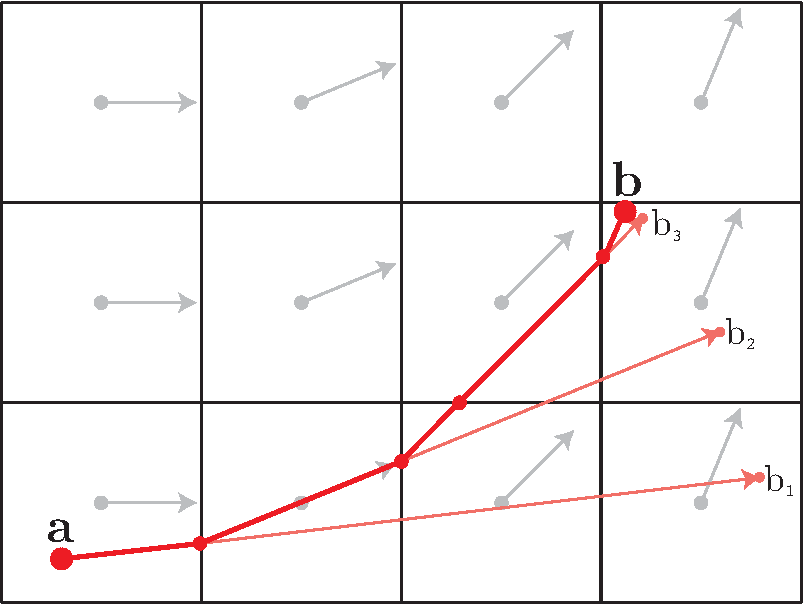
\includegraphics[scale=0.5]{content/gfx/lagrangianSteps.pdf}
  \caption{Two dimensional illustration of a particle trajectory through multiple cells.}
  \label{gfx:lagrangianSteps}
\end{figure}

Figure \ref{gfx:lagrangianSteps} shows a particle which starts at the beginning of a time step at position $\vec{a}$. Its end position is estimated using the velocity field in the cell in which point $\vec{a}$ lies. It is marked as $\vec{b_1}$ in figure 4. After changing the cell the first time, the end position is re-estimated using the velocity field in the new cell. This way the Eulerian time step is broken up into several smaller Lagrangian steps (5 in this example). The thick red line shows the actual trajectory of the particle. The light-red arrows show the estimated end position at the concerning sub steps.

The drag model used to calculate the velocity of the particles in the solidParticle library takes only drag and buoyancy forces into account.

\begin{equation}
    \label{eq:solidParticleVelocity}
    \frac{d \vec{U_p}}{dt} = D_c \cdot | \vec{U_{c}} - \vec{U_{p}} |
        + (1 - \frac{\rho_c}{\rho_p}) \cdot \vec{g}
\end{equation}

Here $\vec{U_p}$ is the velocity of the particle. $\vec{U_c}$ the velocity of the cell in which the particle resides, $\rho_p$ and $\rho_c$ are the densities for the particle and the fluid respectively. The drag coefficient $D_c$ is calculated using the Schiller-Naumann approximation \cite{schillerNaumann}.

\begin{equation}
    \label{eq:solidParticleDrag}        
    D_c = \frac{18}{d^2} \cdot \nu_c \cdot \frac{\rho_c}{\rho_p} 
        \cdot (1 + 0.15 \cdot Re_p^{0.687})
\end{equation}

Here $d$ is the diameter of the particle. The Reynolds number is calculated using the diameter is used $d$ as the characteristic length.

\begin{equation}
    \label{eq:solidParticleRe}
    Re_p = \frac{d}{\nu_c} \cdot | \vec{U_c} - \vec{U_p} |
\end{equation}

\section{GPU Computing}
\label{sec:gpuComputing}

\subsection{Introduction}

Advances in computer graphics and the growth of the video game industry lead to the development of powerful GPUs in the past ten years. It's worth noting that the video game industry generates more revenue than Hollywood nowadays \cite{videogamesRevenue}. While early GPUs were designed to accelerate a fixed graphics pipeline controlled from the CPU, modern GPUs are fully programmable giving the programmer control of the graphics pipeline and allow the execution of small programs, called shaders, directly on the GPU. Developers soon realized that this computing power cannot just be used for graphics, but also to accelerate many problems in computational science. With the release of CUDA in 2007 it became practical to develop computational intense applications for GPUs. Since then thousands of works have been published in which GPUs are used to accelerate computing.

The next two chapters give a short overview of the GPU architecture and the framework used to program GPUs in order to understand the rest of the thesis. For an extensive introduction to GPU programming the author recommends the book  ''Programming Massively Parallel Processors: A Hands-on Approach'' by David B. Kirk and Wen-mei W. Hwu \cite{cudabook} as well as the CUDA C programming guide \cite{cudaguide} which comes with the CUDA software development kit.

\subsection{Architecture of Modern GPUs}
\label{sec:gpuArch}

The performance of modern hardware is largely constrained by the latency of dynamic random access memory (DRAM). While the performance of processors increased greatly, latency of DRAM access did not decrease much, this is often referred to as the memory wall. The reason for this lies in the way how DRAM works: DRAM is basically a very large array of tiny semiconductor capacitors. The presence of a tiny amount of electrical charge distinguishes between 0 and 1. To read the data the charge must be shared with a sensor and if a sufficient amount of charge is present, the sensor detects a 1 (0 otherwise). This is a slow process\footnote{Furthermore DRAM cells must be periodically refreshed otherwise they loose their charge. During refresh cycles the data cannot be accessed.}, the latency for a global memory access is around 400 to 800 clock cycles \cite[5.2.3]{cudaguide} on a GPU.  Modern DRAMs use a parallel process to increase the rate of data: Each time a location is requested many consecutive locations, which include the requested location, are read. Data at consecutive locations can be read at once and then be transferred at high speed to the processor. The programmer must ensure that the program arranges its data in a way that it can be accessed consecutively whenever possible. Otherwise the application will not perform optimally, because more memory transactions than theoretically needed will be executed.

While CPUs are kept busy by using complex automatic caching mechanism\footnote{Around $\frac{1}{3}$ of all transistors are just used for caching in a modern CPU.}, GPUs hide latency using massive parallelism: Thread scheduling on GPUs is implemented in hardware: Each streaming multiprocessor (SM) has its own scheduler. The scheduler bundles threads into warps which are executed simultaneously. If a warp has to wait for data it can be exchanged with another warp ready for calculations. Because scheduling is implemented in hardware dispatching and switching warps has negligible overhead. The SM can automatically coalesce memory access, which is how to the high memory bandwidth advertised \cite[Figure 1.1]{cudaguide} is achieved: If multiple threads in the same warp access consecutive memory locations at the same time hardware coalesces this into a single memory transaction \cite[Appendix F 3.2.1]{cudaguide}. Further vectorized loading of fundamental data types is supported \cite[Table 86]{ptxMan}.

Figure \ref{gfx:fermi} illustrates Nvidia's current architecture named after the Italian physicist Enrico Fermi. Fermi is Nvidia's second generation architecture which supports CUDA. The figure shows a single streaming multiprocessor. The GeForce GTX 470, for example, has 14 multiprocessors and each one has 32 cores\footnote{This explains the warp size of 32.}. The register file is shared among all the threads assigned to an SM. Each thread has it's own register state and program counter, threads can therefore branch independently. However since a warp executes one common instruction at time divergent branching in a wrap is inefficient. Data dependent branches may lead to threads taking different execution paths. In this case both parts a branch are executed sequentially with the concerning threads disabled in either branch \cite[Chapter 4.1]{cudaguide}. Kernels (a program executed on the GPU, see chapter \ref{sec:cuda}) with high register usage limit the number of blocks CUDA can assign to one SM, this may result in poor performance because the scheduler has too few warps to keep the SM busy. To calculate the occupancy of a CUDA program Nvidia provides a spreadsheet \cite{occupancySpreadsheet}. GPUs are often called SIMD (single instruction multiple data) architectures. However compared to SIMD architectures such as Intels SSE (streaming SIMD extension) a GPU offers much more: A scheduler implemented in hardware, state for each threads, independent branching (affects performance, but possible), shared memory, etc. Because of this Nvidia refers to their architecture as \emph{SIMT (single instruction multiple threads)}.

\begin{figure}[H]
  \centering
  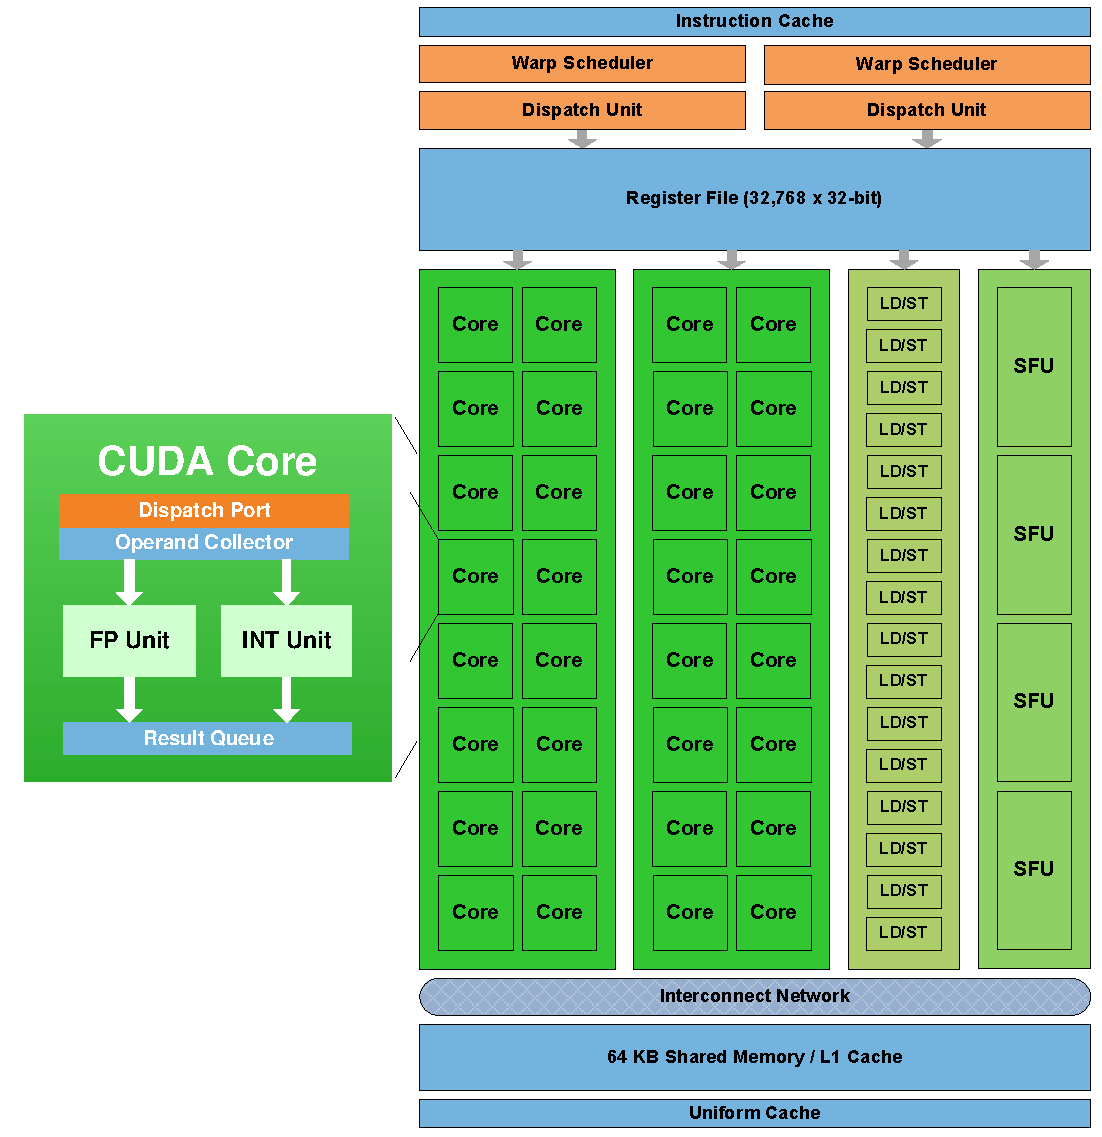
\includegraphics[scale=0.6]{content/gfx/FermiArch.pdf}
  \caption{Nvidia's Fermi architecture, taken from \cite{fermiWhitepaper}.}
  \label{gfx:fermi}
\end{figure}

\subsection{CUDA}
\label{sec:cuda}

CUDA stands for Compute Unified Device Architecture and is a C-style API to program Nvidia's hardware. CUDA is scalable, which means programs written in CUDA can run on any CUDA enabled GPU, independent of the exact hardware configuration. For example the same program can run on a GPU with two streaming multiprocessors or on one with four or eight multiprocessors. However when it comes to performance optimization knowledge of the underlying hardware is often still required.

CUDA defines three key abstractions - a hierarchy of \textbf{thread groups}, \textbf{shared memory} and \textbf{barrier synchronization}. The CUDA terminology differentiates between the host as the CPU executing a host program sequentially and the device (usually a GPU) which executes the CUDA program in parallel. A CUDA host program can allocate memory on the device, copy data between the host and the device and execute programs on the GPU. Programs running on the GPU are called \textbf{kernels}. A kernel must be configured when it is called, meaning that the programmer must specify on how many threads blocks the kernel runs and the number of threads per block. Kernels are defined and invoked using a proprietary syntax \cite[2.1]{cudaguide}. CUDA source files usually end with \verb+cu+ and can include a mix of host and device code. During the compilation workflow the host code is separated from the device code. The device code is compiled into assembly form, and the host code is passed on to the concerning compiler (for example \verb+g+++ on a Linux environment) \cite[3.1]{cudaguide}.
\section{Software Development}

\label{sec:coding}

\subsection{Software Design}

The engine for particle tracking on the GPU is built upon the solid particle library. A solver called \verb+gpuLagrangianFoam+ was developed. If it is invoked using the \verb+-gpu+ switch, tracking will be executed on the GPU. Because CUDA files must be compiled using Nvidia's proprietary compiler, \verb+nvcc+, the code using CUDA keywords was developed as a separate shared library against which the solver must be linked. The rest of the solver code can be compiled in the same way as any other OpenFOAM application.

\paragraph{Mesh Data}

As explained earlier, the OpenFOAM \verb+Cloud+ class stores particles in a linked list, which is not suitable for parallel processing on a GPU. Before the mesh can be used on the GPU, it is converted into a more suitable format, which is described here. Three dimensional vectors are padded to 4 elements such that they can be fetched using CUDA's built in vector data types \verb+float4+ or \verb+double4+. For example, the cell centres are stored by the order of cell labels as illustrated in figure \ref{gfx:cellCentres}.

\begin{figure}[H]
  \centering
  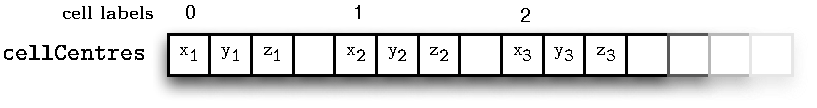
\includegraphics[scale=0.8]{content/gfx/cellCentres.pdf}
  \caption{Cell centres arranged in memory.}
  \label{gfx:cellCentres}
\end{figure}

The cell labels are not stored, since they go from $0$ to the number of cells $- 1$. Storing the face labels associated with the cell labels requires some more effort because in an unstructured mesh a cell can have any number of faces. 

\begin{figure}[H]
  \centering
  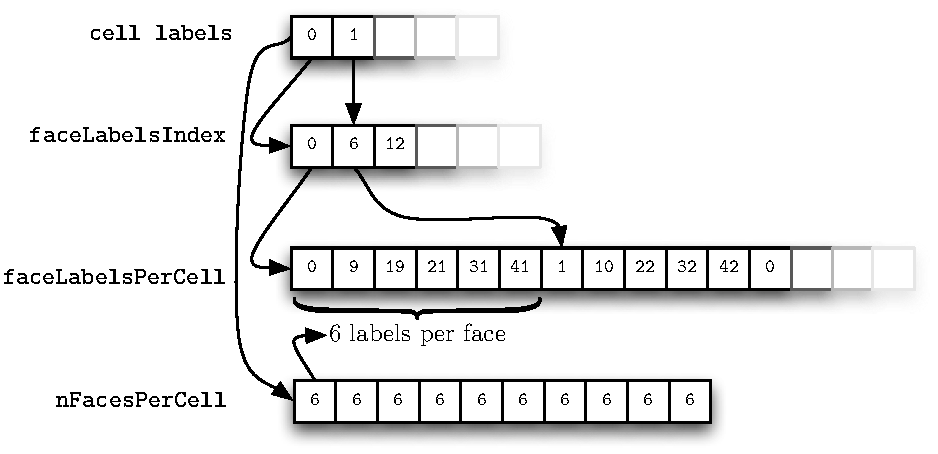
\includegraphics[scale=0.8]{content/gfx/cellFacesMapping.pdf}
  \caption{Mesh data layout in memory.}
  \label{gfx:cellFacesMapping}
\end{figure}

Figure \ref{gfx:cellFacesMapping} illustrates the mapping from the cell labels to the concerning face labels. The face labels are stored in the array \verb+faceLabelsPerCell+, by cell. Meaning that the first six face labels belong to cell \verb+0+ and the next six to cell \verb+1+. Face label \verb+0+ appears twice, this is the label of the face between cell \verb+0+ and \verb+1+. The \verb+faceLabelsIndex+ array stores the indices of the \verb+faceLabelsPerCell+ array, where the face labels to a given cell start. Note that the array names are identically to the ones used in the code. The mesh data was taken from the tunnel test case (see section \ref{sec:particleTunnel}), which consists of ten cubes placed one after another. Data belonging to a certain face, such as the face centres and the face normals are stored at the same index as the face labels. The neighbour and owner arrays are implemented as described in section \ref{sec:meshRepresentation}. This is illustrated in figure \ref{gfx:ownerNeighbour}, the data is again taken from the particle tunnel case. There are only ten faces with a neighbour cell: Face 0 has neighbour cell 1, face 1 neighbour cell 2 and so forth. 

\begin{figure}[H]
  \centering
  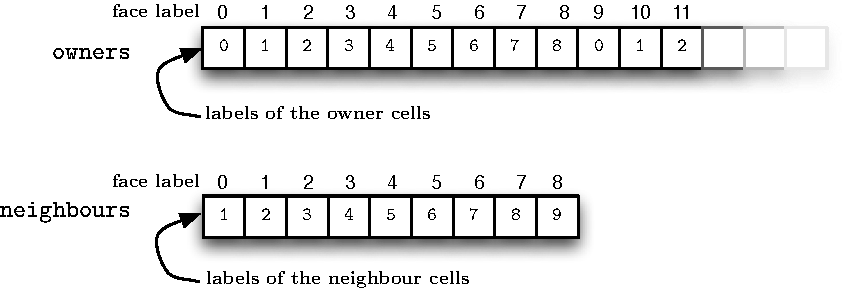
\includegraphics[scale=0.8]{content/gfx/ownerNeighbour.pdf}
  \caption{Owner and neighbour data of the particle tunnel case.}
  \label{gfx:ownerNeighbour}
\end{figure}

\paragraph{Particle Data}

The particle data is stored in a similar fashion as the mesh data. For example the labels of the faces for which $\lambda_c$ is in the interval $[0,1]$ (see section \ref{sec:particleTrackingAlgo}) also use an additional index array.

\paragraph{Abstraction and Data Encapsulation}

When programming CUDA, the host code can be completely written in C++ while only C code with a few extensions borrowed from C++ such as operator overloading or function templates \cite[Appendix D]{cudaguide} is allowed on the device. This makes it impossible to use containers from the C++ standard template library (STL) or OpenFOAM classes on the device. Using only manually allocated arrays in order to manage the data often leads to error prone code and therefore long testing and debugging time. To transform the data into a flat structure, suitable for the GPU, the vector container from the STL was used. The C++ ISO standard guarantees that the data is stored contiguously in memory such that it can be copied to the GPU using raw pointers. From the C++ standard document \cite[23.3.6.1]{cpp}:

\begin{quote}
The elements of a vector are stored contiguously, meaning that if \verb+v+ is a \verb+vector<T, Allocator>+ where \verb+T+ is some type other than bool, then it obeys the identity \verb@&v[n] == &v[0] + n@ for all \verb@0 <= n < v.size()@.
\end{quote}

The classes of the GPU particle engine use a wrapper which holds a reference to the concerning instance of \verb+std::vector+ and a pointer to the device memory as member variables. The wrapper class is called \verb+cuvector+. Device memory is allocated upon construction and freed when the destructor is called. Memory can be copied from the host to the device calling \verb+upload()+ on the cuvector object, \verb+download()+ is used to copy the data back from the device to the host memory. The code of the particle tracking engine is divided into three major classes: The \verb+FlatMesh+ class holds all the mesh data and does basic operations on it, such as figuring out what the cell next to another cell is, given a cell and a face label. The \verb+ParticleData+ class holds all particle related data. Finally the \verb+particleEngine+ class is derived from the \verb+ParticleData+ class and does the actual computation, such as computing all the $\lambda_c$ and the $\lambda_a$. It also moves particles and keeps track of how many particle do still need tracking. Figure \ref{gfx:engineOverview} illustrates these classes briefly.

\begin{figure}[H]
  \centering
  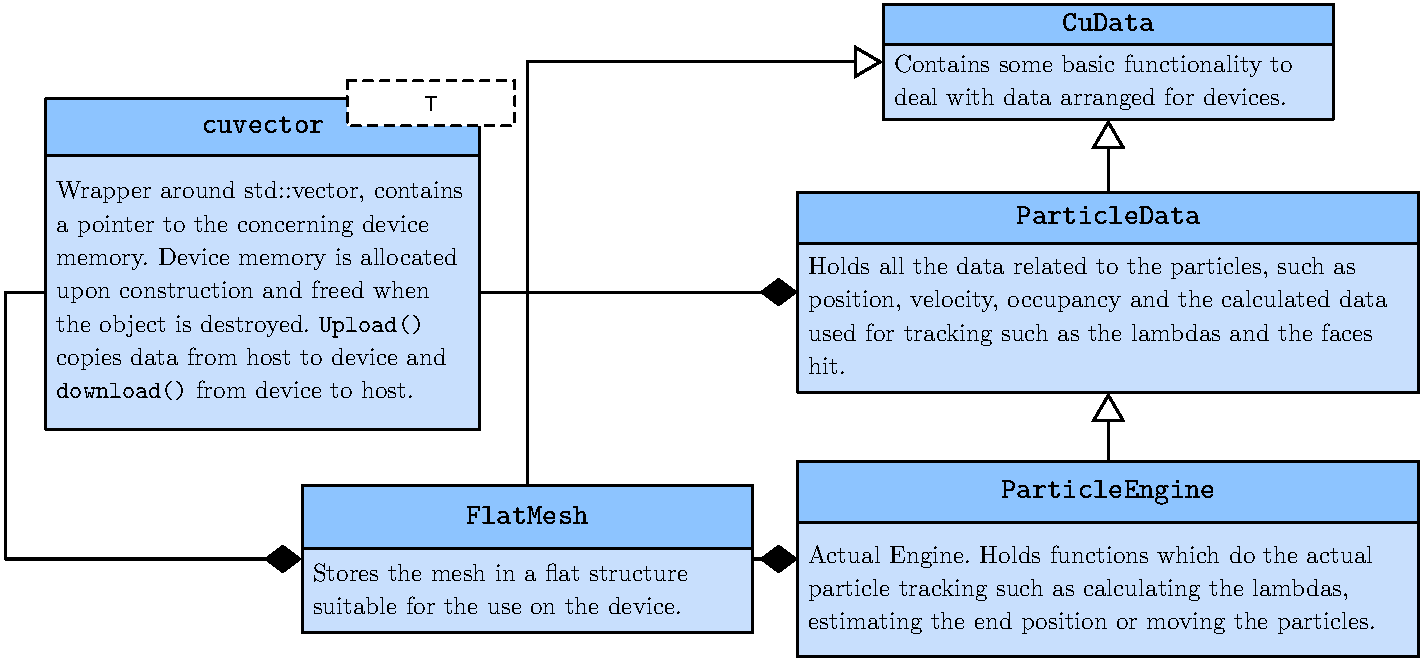
\includegraphics[scale=0.6]{content/gfx/ParticleEngineOverview.pdf}
  \caption{Simplified class diagram of the GPU tracking library.}
  \label{gfx:engineOverview}
\end{figure}

\subsection{Complete Particle Engine}

Tracking a set of particles given a start position and an (estimated) end position involves several steps. First one needs to calculate $\lambda_c$ for all particles. Recalling the equation (\ref{eq:4}) for $\lambda_c$

\begin{eqnarray}
    \lambda_{c} = \frac{(\vec{C_f} - \vec{C_c}) \bullet \vec{S_f}}{(\vec{b} - \vec{C_c}) \bullet \vec{S_f}} \nonumber
\end{eqnarray}

The only data depending on the particle to track is the end position $\vec{b}$. Therefore we can calculate the numerator of (\ref{eq:4}) in advance for every face and cell. This is done right after the mesh data is uploaded. Once $\lambda_c$ is calculated, we have a set of faces for every particle, the faces for which $\lambda_c$ is in the interval $[0,1]$. This set usually consists of zero, one or two faces.\footnote{More faces per particle can be found, but this happens not very often.} Particles for which no face was found have their end position inside the same cell in which they were at the beginning. All we need to do is move them to the end position. Therefore we need to resort the particle data and create a second set consisting of particles which still need tracking, we call this the set of remaining particles. For those, $\lambda_a$ must be calculated to figure out which face they hit. With this information all the particles can be moved: Particles not in the set of remaining particles can be moved to the end. For particles in the set of remaining particles it must be checked whether the face hit is a boundary face, and if so, the particle must be reflected at the boundary. Otherwise the particle is moved onto the face hit and the occupancy information is updated to the adjacent cell. In the next step only particles in the remaining set of this step need to be considered. Before starting with the next iteration, the velocity must be updated using the velocity vector of the new occupancy cell. This process is illustrated in figure \ref{gfx:SequenceTracking}.

\begin{figure}[H]
  \centering
  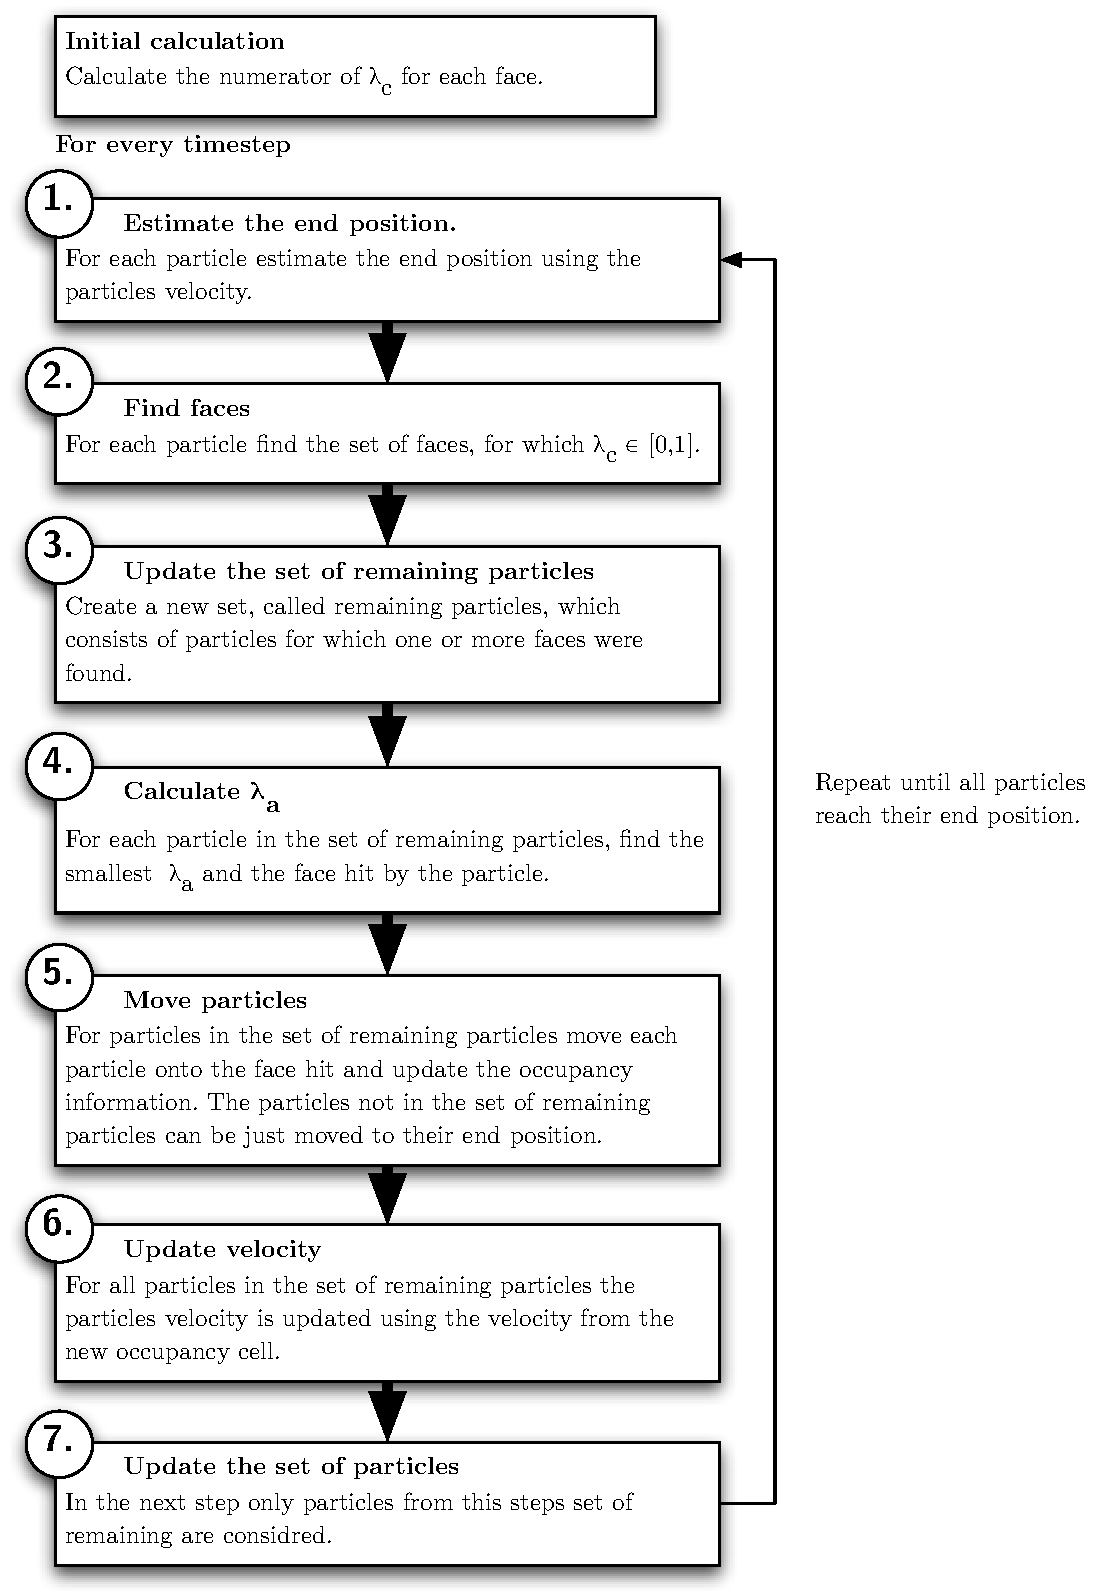
\includegraphics[scale=0.8]{content/gfx/SequenceTracking.pdf}
  \caption{Complete particle tracking sequence.}
  \label{gfx:SequenceTracking}
\end{figure}

\subsection{Data Reduction}

After calculating $\lambda_c$ it is known which particles stay in their cell. The set of particles is then reduced to the set of remaining cells using the array which holds the number of faces found as illustrated in figure \ref{gfx:reduce}.

\begin{figure}[H]
  \centering
  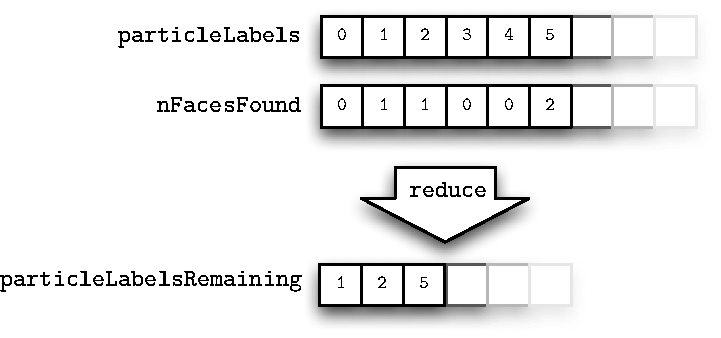
\includegraphics[scale=0.8]{content/gfx/reduce.pdf}
  \caption{Reducing the particle labels array to those which sill need tracking.}
  \label{gfx:reduce}
\end{figure}

When programming sequentially, this can be done with one simple loop. Copying the data back from the device to the host, then sort it in just one thread and upload it again takes far too much time. This is illustrated in figure \ref{gfx:widthPlotGapSort}, where the runtime of all kernel functions and memory coping is plotted. In this test, the total computing time spent on the GPU is just around 15\%. A huge part is used to copy the memory between the host and the device. The white gap shows that the GPU is idle during the time spent on the host to reduce data. The test was done on the torus (see section \ref{sec:torus}) case, where the lambdas for 100'000 particles were calculated .

\begin{figure}[H]
  \centering
  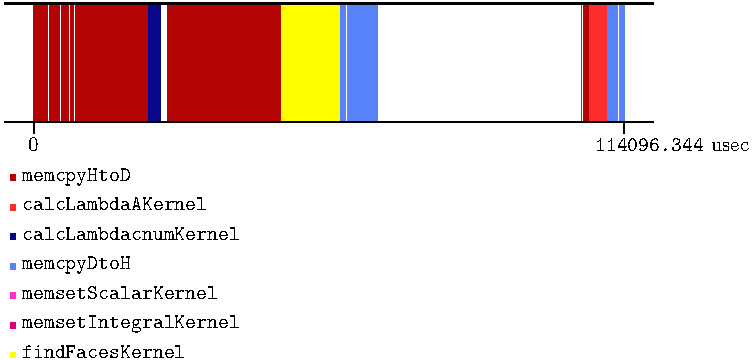
\includegraphics[scale=0.8]{content/gfx/widthPlotGapSort.pdf}
  \caption{Width plot of the GPU time spent for calculating lambdas. The CPU is used for data reduction.}
  \label{gfx:widthPlotGapSort}
\end{figure}

Doing such a reduction efficiently on massively parallel hardware is far less trivial. Fortunately sorting on the GPU is already implemented \cite{thrustRadixSort}. Thrust \cite{thrust} is a library of basic algorithms for the GPU with an interface similar to the standard template library. It includes algorithms for counting, sorting and searching. The particle labels array is reduced by the following steps on the GPU.

\begin{enumerate}
    
    \item Count the number of zeros in \verb+nFacesFound+. Use this to calculate how many particles still remain.
    
    \item Sort the \verb+particleLabels+ array using the \verb+nFacesFound+ array as key in descending order. All the labels with no faces hit will be at an index greater or equal to the number of particles remaining.
    
\end{enumerate}

\subsection{Tools and Validation}

In order to validate the results \verb+solidParticleFoam+ has been modified so that all the data going through the \verb+trackToFace(..)+ is written to the disc in binary\footnote{In a first attempt the data was just written out in text format. Because of the loss of precision it was difficult to compare the results again.} format. This includes the beginning and the end position of each particle, the cell it occupies at the beginning, the face it hits (if any) and the lambdas calculated. This data is then read by a test program, which calculates the lambdas and the faces hit again on the GPU using the start and end position stored before. The results are then compared and any differences between them is reported. This utility is called \verb+calcLambdas+ and requires the \verb+-data <dataDir>+ argument.

Doing so validates the results of the kernels which are responsible to calculate the lambdas, step 2, 3 and 4 in figure \ref{gfx:SequenceTracking}, but whether the particles are moved correctly or not is not verified. The \verb+gpuLagrangianFoam+ utility therefore comes with a switch called \verb+-validate+. If it is turned on the mesh is searched after moving the particles at the end of the time step in order to verify that the particles are in the correct cell. To generate a number of particles as test data a utility called \verb+genRandCloud+ was developed. It takes the desired number of particles as input argument and randomly positions particles in the simulation domain.

Searching the mesh is done using the octree library \cite{octree} OpenFOAM provides: The problem of finding the correct cell, given a position is reduced to the nearest neighbour problem. The centroids of all the cells in a mesh are taken as point-set and the position of the particle as the query point. The probability that the particle is in the same cell as the closest centroid is quite high and if it is not, it will be in one of the neighbouring cells. The octree is used for spatial subdivision: The bounding box of the simulation domain is recursively subdivided into 8 smaller boxes, starting from the center of the bounding box. Recursion stops once all centroids are in a separate box. During this process a tree is built which contains the direction for each step. This can be explained easier in two dimensions: Where the bounding box would be divided into 4 rectangles one at the north west, south west, north east and south east. Using this tree the program just needs to follow the direction given a position in order to solve the nearest neighbour problem.
\section{Test Cases and Results}
\label{sec:results}

\subsection{Tunnel}
\label{sec:particleTunnel}

The tunnel test case is very simple and was mainly used for debugging during development. It consists of ten cubes. This is illustrated in figure \ref{fig:particleTunnel} the particles are colored by the x-coordinate (goes from left to right in the illustration) of their velocity.

\textbf{\begin{figure}[H]
  \centering
  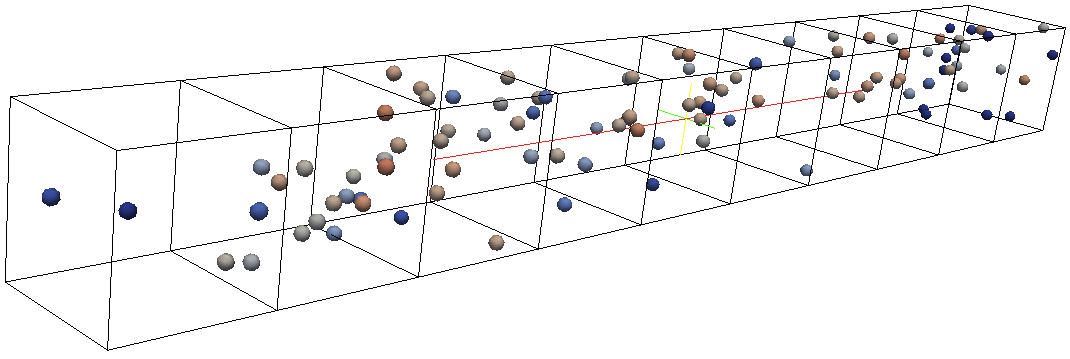
\includegraphics[scale=0.4]{content/gfx/particleTunnel.png}
  \caption{Particle tunnel with randomly distributed particles.}
  \label{fig:particleTunnel}
\end{figure}}

\subsection{Torus}
\label{sec:torus}

The second test case is a simple torus. A torus is defined by two circles orthogonal to each other in three dimensional space. The smaller circle is then rotated around the bigger circle leading to a surface of revolution which defines the torus.

\textbf{\begin{figure}[H]
  \centering
  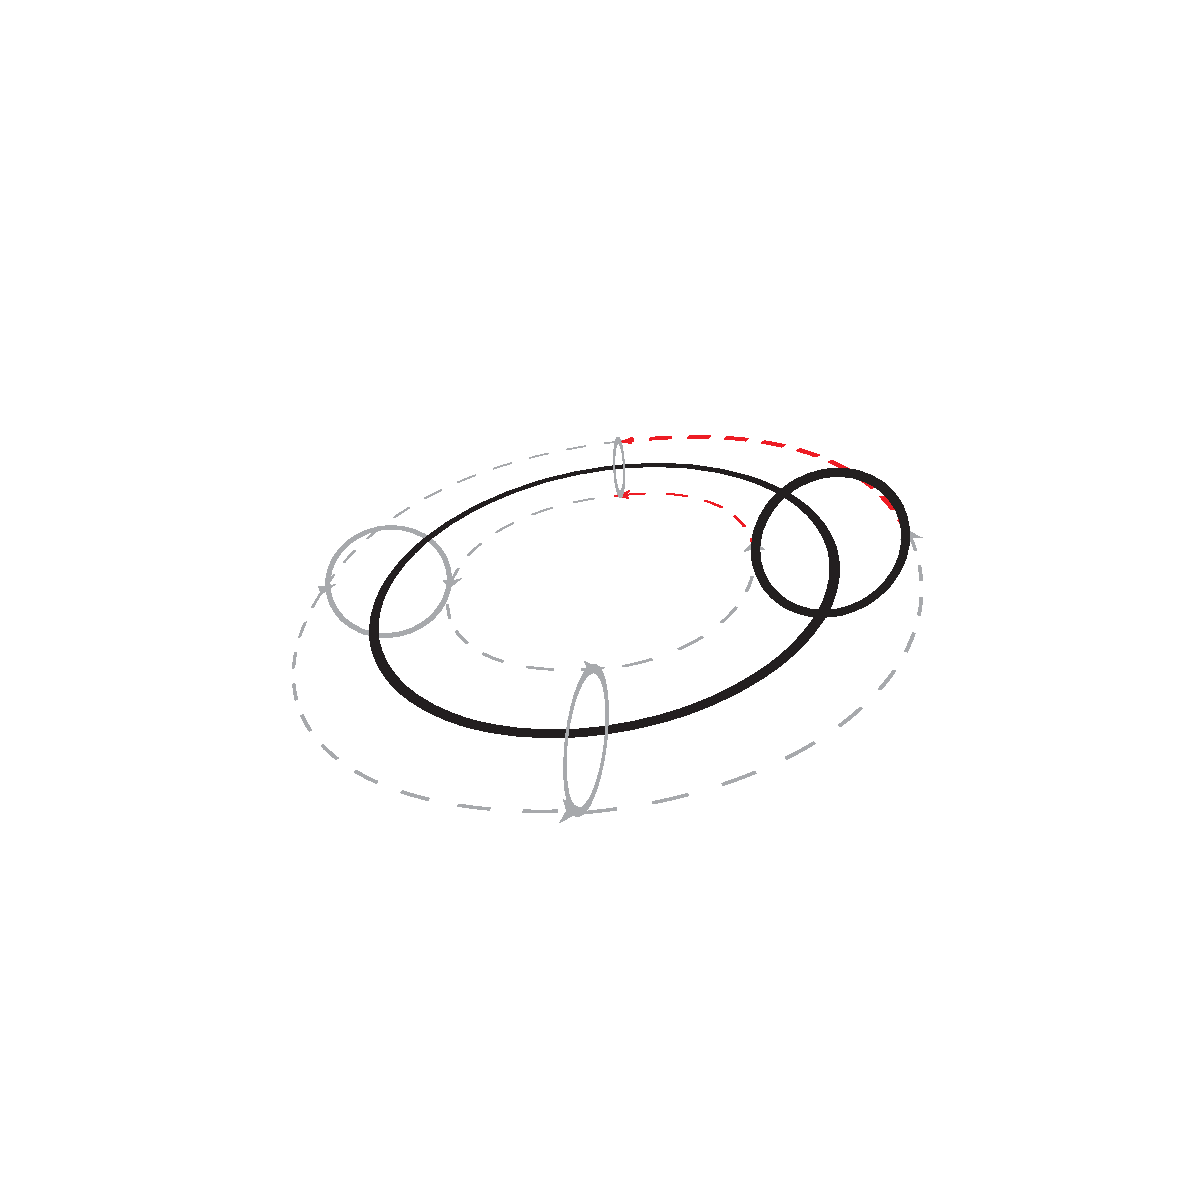
\includegraphics[scale=0.8]{content/gfx/torus.pdf}
  \caption{A torus defined by surface revolution of a circle.}
  \label{fig:torus}
\end{figure}}

In order to polygonally approximate the torus discrete points on the rotating circle are calculated using formula \ref{eq:torus}. The formula requires the following parameters: $(x_0, y_0)$ is the center of the circle, $r$ is the radius of the circle and $(x, y)$ the points lying on the circle.

\begin{equation}
    \label{eq:torus}
    (x, y) = (x_0 + r \cdot cos(\alpha), y_0 + r \cdot sin(\alpha))
\end{equation}

% TODO figure explaining the discretisation

The mesh was then generated using netgen \cite{netgen}, a simple mesh generator which can export meshes in the OpenFOAM format.

\textbf{\begin{figure}[H]
  \centering
  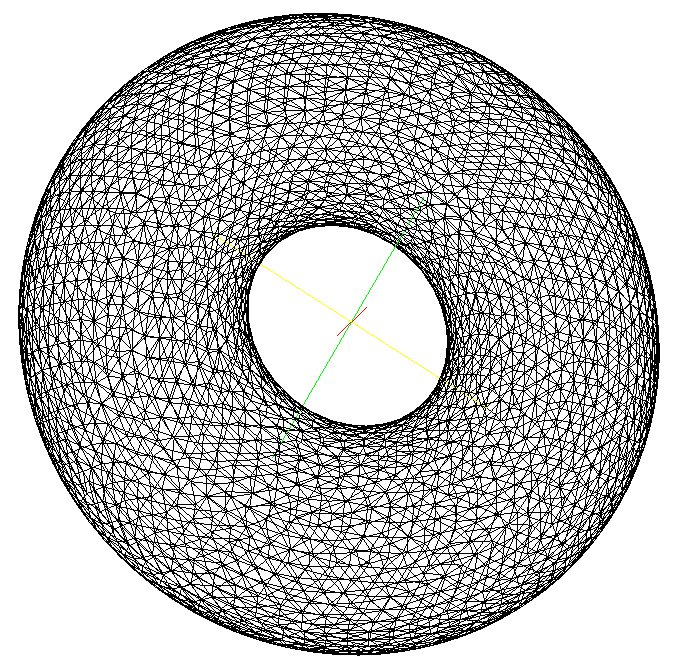
\includegraphics[scale=0.4]{content/gfx/torusCoarseMesh.png}
  \caption{A tetrahedral mesh generated in a torus.}
  \label{gfx:torus}
\end{figure}}

Figure \ref{gfx:torus} shows a coarse mesh with around 30000 cells generated in  a torus.

\subsection{Measurements}

The performance measurements are done using the torus case with 228'184 cells. The tests ran on an Intel 655k CPU\footnote{\url{http://ark.intel.com/Product.aspx?id=48750}} and an Nvidia GeForce GTX 470\footnote{\url{http://www.nvidia.com/object/product_geforce_gtx_470_us.html}}. Both parts have been released to the market in 2010. 50'000 particles are tracked over ten time steps, which is equivalent to calculating the lambdas for 500'000 particles.

\begin{table}[H]
    \centering
    \begin{tabular}{| l | l | l |}
        \hline
                          & \textbf{CPU} & \textbf{GPU} \\ \hline
        Single Precision  & 2'810'792    &  220'866 \\ \hline
        Double Precision  & 3'264'259    &  376'349 \\ \hline
    \end{tabular}
    \caption{Execution time in microseconds}
    \label{table:execTime}
\end{table}

Table \ref{table:execTime} compares the time required to calculate the lambdas on the CPU using the OpenFOAM code and on the GPU using the code developed during this thesis. It should be noted that the GPU time includes the time required to copy all the data over the PCI bus and that the actual computing time on the GPU is much shorter! Because of this tracking particles on the GPU only makes sense for a larger number of particles as illustrated by figure \ref{gfx:plotGpuVSCpu}. 

\textbf{\begin{figure}[H]
  \centering
  % GNUPLOT: LaTeX picture with Postscript
\begingroup
  \makeatletter
  \providecommand\color[2][]{%
    \GenericError{(gnuplot) \space\space\space\@spaces}{%
      Package color not loaded in conjunction with
      terminal option `colourtext'%
    }{See the gnuplot documentation for explanation.%
    }{Either use 'blacktext' in gnuplot or load the package
      color.sty in LaTeX.}%
    \renewcommand\color[2][]{}%
  }%
  \providecommand\includegraphics[2][]{%
    \GenericError{(gnuplot) \space\space\space\@spaces}{%
      Package graphicx or graphics not loaded%
    }{See the gnuplot documentation for explanation.%
    }{The gnuplot epslatex terminal needs graphicx.sty or graphics.sty.}%
    \renewcommand\includegraphics[2][]{}%
  }%
  \providecommand\rotatebox[2]{#2}%
  \@ifundefined{ifGPcolor}{%
    \newif\ifGPcolor
    \GPcolortrue
  }{}%
  \@ifundefined{ifGPblacktext}{%
    \newif\ifGPblacktext
    \GPblacktexttrue
  }{}%
  % define a \g@addto@macro without @ in the name:
  \let\gplgaddtomacro\g@addto@macro
  % define empty templates for all commands taking text:
  \gdef\gplbacktext{}%
  \gdef\gplfronttext{}%
  \makeatother
  \ifGPblacktext
    % no textcolor at all
    \def\colorrgb#1{}%
    \def\colorgray#1{}%
  \else
    % gray or color?
    \ifGPcolor
      \def\colorrgb#1{\color[rgb]{#1}}%
      \def\colorgray#1{\color[gray]{#1}}%
      \expandafter\def\csname LTw\endcsname{\color{white}}%
      \expandafter\def\csname LTb\endcsname{\color{black}}%
      \expandafter\def\csname LTa\endcsname{\color{black}}%
      \expandafter\def\csname LT0\endcsname{\color[rgb]{1,0,0}}%
      \expandafter\def\csname LT1\endcsname{\color[rgb]{0,1,0}}%
      \expandafter\def\csname LT2\endcsname{\color[rgb]{0,0,1}}%
      \expandafter\def\csname LT3\endcsname{\color[rgb]{1,0,1}}%
      \expandafter\def\csname LT4\endcsname{\color[rgb]{0,1,1}}%
      \expandafter\def\csname LT5\endcsname{\color[rgb]{1,1,0}}%
      \expandafter\def\csname LT6\endcsname{\color[rgb]{0,0,0}}%
      \expandafter\def\csname LT7\endcsname{\color[rgb]{1,0.3,0}}%
      \expandafter\def\csname LT8\endcsname{\color[rgb]{0.5,0.5,0.5}}%
    \else
      % gray
      \def\colorrgb#1{\color{black}}%
      \def\colorgray#1{\color[gray]{#1}}%
      \expandafter\def\csname LTw\endcsname{\color{white}}%
      \expandafter\def\csname LTb\endcsname{\color{black}}%
      \expandafter\def\csname LTa\endcsname{\color{black}}%
      \expandafter\def\csname LT0\endcsname{\color{black}}%
      \expandafter\def\csname LT1\endcsname{\color{black}}%
      \expandafter\def\csname LT2\endcsname{\color{black}}%
      \expandafter\def\csname LT3\endcsname{\color{black}}%
      \expandafter\def\csname LT4\endcsname{\color{black}}%
      \expandafter\def\csname LT5\endcsname{\color{black}}%
      \expandafter\def\csname LT6\endcsname{\color{black}}%
      \expandafter\def\csname LT7\endcsname{\color{black}}%
      \expandafter\def\csname LT8\endcsname{\color{black}}%
    \fi
  \fi
  \setlength{\unitlength}{0.0500bp}%
  \begin{picture}(7200.00,5040.00)%
    \gplgaddtomacro\gplbacktext{%
      \csname LTb\endcsname%
      \put(1474,704){\makebox(0,0)[r]{\strut{} 0}}%
      \put(1474,1229){\makebox(0,0)[r]{\strut{} 500000}}%
      \put(1474,1754){\makebox(0,0)[r]{\strut{} 1e+06}}%
      \put(1474,2279){\makebox(0,0)[r]{\strut{} 1.5e+06}}%
      \put(1474,2804){\makebox(0,0)[r]{\strut{} 2e+06}}%
      \put(1474,3329){\makebox(0,0)[r]{\strut{} 2.5e+06}}%
      \put(1474,3854){\makebox(0,0)[r]{\strut{} 3e+06}}%
      \put(1474,4379){\makebox(0,0)[r]{\strut{} 3.5e+06}}%
      \put(1606,484){\makebox(0,0){\strut{} 0}}%
      \put(2126,484){\makebox(0,0){\strut{} 5}}%
      \put(2645,484){\makebox(0,0){\strut{} 10}}%
      \put(3165,484){\makebox(0,0){\strut{} 15}}%
      \put(3685,484){\makebox(0,0){\strut{} 20}}%
      \put(4205,484){\makebox(0,0){\strut{} 25}}%
      \put(4724,484){\makebox(0,0){\strut{} 30}}%
      \put(5244,484){\makebox(0,0){\strut{} 35}}%
      \put(5764,484){\makebox(0,0){\strut{} 40}}%
      \put(6283,484){\makebox(0,0){\strut{} 45}}%
      \put(6803,484){\makebox(0,0){\strut{} 50}}%
      \put(176,2541){\rotatebox{-270}{\makebox(0,0){\strut{}Time in Microseconds}}}%
      \put(4204,154){\makebox(0,0){\strut{}Number of Particles (times 10'000)}}%
      \put(4204,4709){\makebox(0,0){\strut{}CPU vs GPU}}%
    }%
    \gplgaddtomacro\gplfronttext{%
      \csname LTb\endcsname%
      \put(5816,4206){\makebox(0,0)[r]{\strut{}CPU}}%
      \csname LTb\endcsname%
      \put(5816,3986){\makebox(0,0)[r]{\strut{}GPU}}%
    }%
    \gplbacktext
    \put(0,0){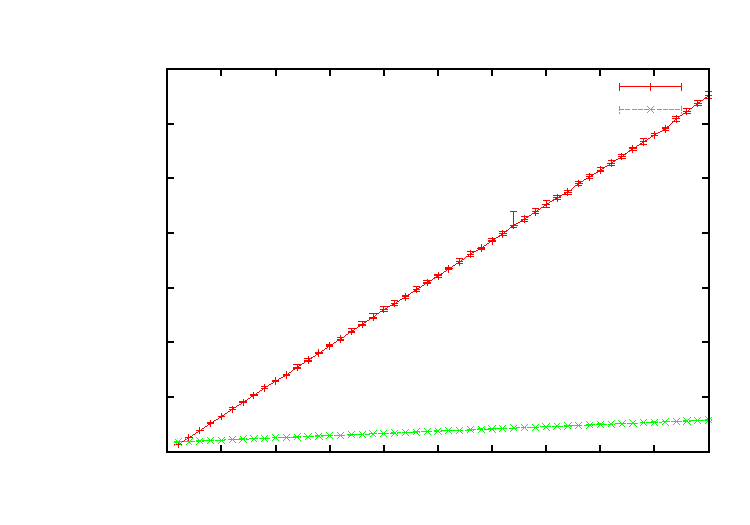
\includegraphics{content/gfx/gpuVsCpu}}%
    \gplfronttext
  \end{picture}%
\endgroup

  \caption{Plot showing the execution time for a growing number of particles.}
  \label{gfx:plotGpuVSCpu}
\end{figure}}

The execution times in figure \ref{gfx:plotGpuVSCpu} have been measured ten times at each point. For each point the average, the highest and lowest time is shown, the average values are connected by lines. As one can see there are some measurement errors on the CPU, this is most likely because the operating system and further user processes are running on the CPU along with the OpenFOAM code. On the GPU only very little diversity in the measurements can be seen, this is because the test was running on a dedicated GPU, not used for graphics.

For a more detailed analysis of the computing time spent on the GPU Nvidia's Compute Profiler \cite{computeprof} was used.

\textbf{\begin{figure}[H]
  \centering
  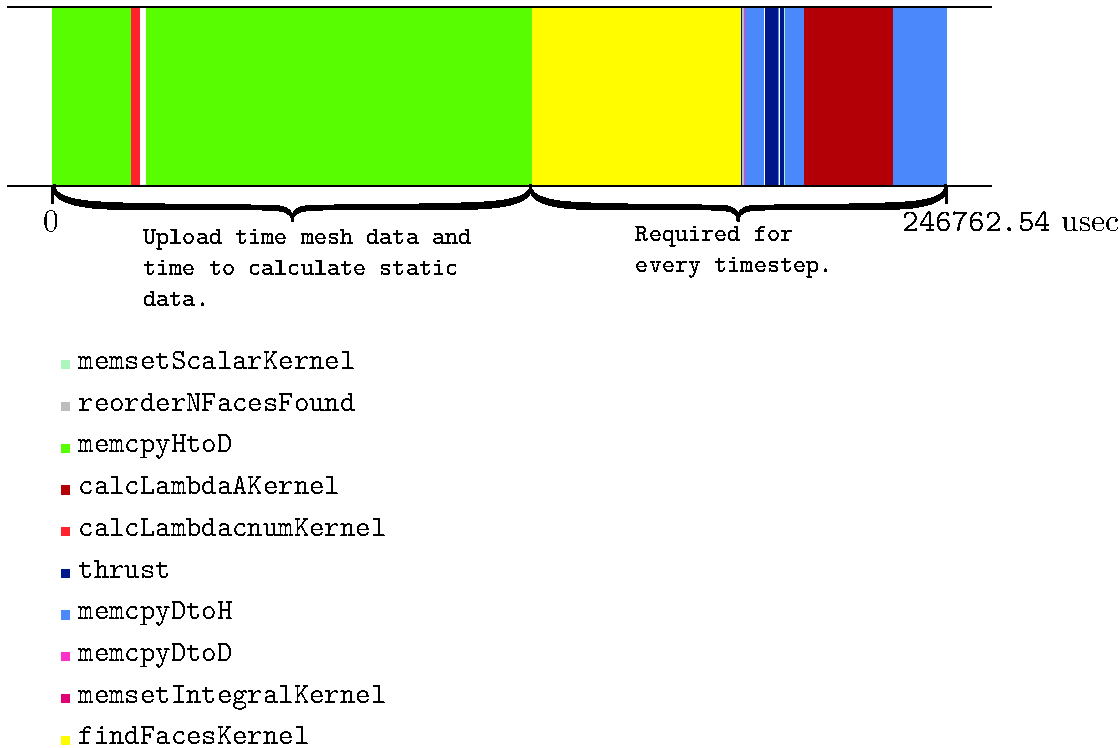
\includegraphics[scale=0.6]{content/gfx/widthPlot1.pdf}
  \caption{Width plot showing the time of kernel functions and memcpy operations.}
  \label{fig:widthPlot}
\end{figure}}

Figure \ref{fig:widthPlot} shows a width plot of the GPU time\footnote{The plot was done using the same test case (with double precision) as presented before in table \ref{table:execTime}. The shorter time is because this is a sum of time measured on the GPU (for copying data and GPU kernels), while the time presented in the table was measured on the CPU and therefore includes overhead for invoking memory copies and GPU kernels.}. The white spaces in between indicate idle time in which the host code is doing something. It can be easily seen that around 60 \% of the run time are memory copying time! Furthermore the first chunk of data copied is the mesh data. This together with the initial calculation must be done only once.

\textbf{\begin{figure}[H]
  \centering
  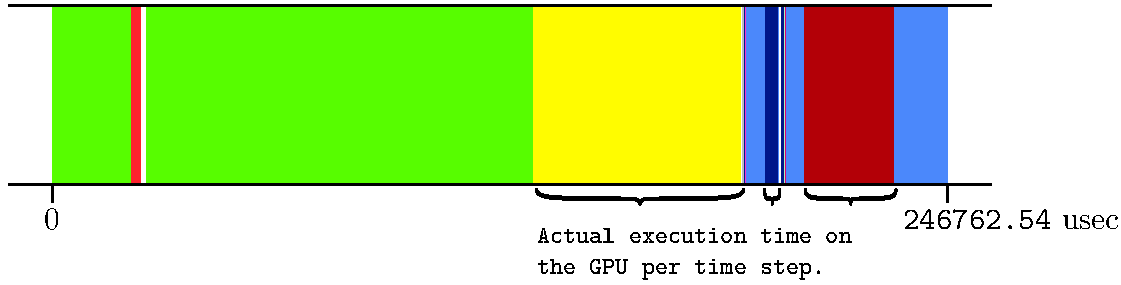
\includegraphics[scale=0.6]{content/gfx/widthPlotAcutalExecutionTimeGPU.pdf}
  \caption{Width plot showing the actual time spent on the GPU.}
  \label{fig:widthPlotAcutalTimeGPU}
\end{figure}}

If we do not consider the time spent to copy the data over the PCI bus and to do the initial calculation, then we get an actual run time on the GPU of just 89'742 usec per time step (double precision). \textit{That is more than 30 times faster than the single threaded CPU implementation.} The actual execution time on the GPU is illustrated in figure \ref{fig:widthPlotAcutalTimeGPU}.

\subsection{Performance Analysis of Computational Kernels}

There are three major kernels involved in the computation: A kernel which calculates the numerator of $\lambda_c$ at the beginning (initial step in figure \ref{gfx:SequenceTracking}), this kernel has one thread per cell. A kernel which finds all faces with $\lambda_c \in [0, 1]$ (step 2 in figure \ref{gfx:SequenceTracking}) with one thread per particle and a kernel which calculates $\lambda_a$ for the particles with $\lambda_c \in [0, 1]$\footnote{The kernels to calculate the lambdas are parallelized over the number of particles. It would also be possible to parallelize over all the cells in the mesh but this would require that each thread iterates over the particles in its cell. Because the number of particles per cell usually varies this would lead to massively divergent warps and therefore poor performance \cite[5.4.2]{cudaguide}} (step 4 in figure \ref{gfx:SequenceTracking}). 

Because the kernel responsible for finding faces with $\lambda_c \in [0,1]$ takes the most time to compute (figure \ref{fig:widthPlot}, yellow) it is analysed here. The structure of the kernel is as follows: First data belonging to the cell and the particle is fetched using the particle label. Then it is iterated over all faces of the cell where first the face data (face normal and face centre) is fetched and then the lambdas are calculated. If they are within the desired interval the label of the face is written into the faces found array. Once the loop is done the number of faces found is written back. When compiled for double precision the kernel's occupancy (see section \ref{sec:gpuArch}) is quite low around 33\%, this is because each thread requires 34 registers. Compiled for single precision improves the occupancy (around 66\%), because just 24 registers are required. In both cases the occupancy is limited by register usage. If it could be done with just 16 registers per thread, the occupancy would be 100 \%. The kernel is memory bound, meaning that execution time is wasted by waiting for data from global memory. The main reason for this are uncoalesced reads and writes as well as the low occupancy. For example writing the face labels found is uncoalesced because it differs for every thread and therefore it is written back sequentially. There are different options to further improve the kernel's efficiency

\begin{itemize}
    \item Turn off L1 cache for global memory access. Uncached memory transactions are multiples of 32, 64 and 128 bytes where cached transactions are always multiples of 128 bytes (the cache line size) \cite[F.4.2]{cudaguide}. In case of uncoalesced memory access, smaller transactions are better, because the full size of the cache line is not used anyways. Quickly trying this out lead to a slight improvement of around 20\%\footnote{The plots presented before are with L1 cache enabled.}.
    \item Use shared memory or texture cache. Shared memory is fast, on-chip memory, which can be accessed by threads in the same block \cite[3.2.3]{cudaguide}. However tracking particles in an unstructured mesh is not well suited for shared memory: Using shared memory requires that threads sharing data are placed in the same CUDA block. The threads for the particles which reside in the same cell share data: The cell centre, face centres and normals, etc. However this would require that the particles are sorted by the occupancy cells. Also all CUDA blocks for a kernel launch must be of the same size. Furthermore the block size should be a multiple of the wrap size (32 threads) and at minimum 64 threads \cite[4.4]{cudaBestPractices}. This makes it unfeasible to use shared memory. Using texture memory \cite[3.2.10.1]{cudaguide} might speed up the kernel, since it lead to significant performance improvement in Nvidia's particle demo (see section \ref{sec:summary}).
    \item Review the code and rearrange data in order to improve memory access patterns and reduce the register requirements. The kernel code first fetches the label of the particles. During the first iteration the label of the particles correspond directly to the thread index. The particle labels array is just used in later iterations, where some particles are already done. Because the number of particles which need to be considered in further iterations are usually much smaller, this could lead to a significant improvement. 
\end{itemize}

\subsection{Memory Requirements}

GPUs have memory buses designed to reduce latency and not to support a very large amount of memory as CPUs do. To day GPUs can have at most 6GB of RAM. For larger cases it is probably required to partition the particles into chunks fitting into the memory of the GPU.

In the simulation code a particle requires about 1338 bytes of memory to store all the relevant data (position, velocity, diameter, label, etc). Therefore processing one million particles at once would require around 1.25 Gb of memory just for the particles. A tetrahedral mesh cell requires about 221 bytes of memory. A mesh with one million cells therefore requires about 212 Mb of data. The \verb+calcLambda+ test program and the \verb+gpuLagrangianFoam+ solver report the data required on the GPU at the beginning of the simulation.
\section{Conclusion and Future Work}

It was shown that the Lagrangian particle tracking algorithm can run efficiently on the GPU. Porting it required the conversion of the mesh data into structures suitable for the SIMT architecture. The algorithm itself could be parallelized easily since the computations are done for each particle individually which is well suitable for massively parallel processors. The biggest problem, with respect to efficiency, are the time consuming memory copies over the PCI bus. Having to copy data over a slow bus repeatedly can nullify speedups achieved by porting parts of a simulation to massively parallel hardware. While there exist several workarounds, such as the possibility to overlap copying with kernel execution, the problem will probably be gone in future hardware generations. For example Advanced Micro Devices (AMD) already announced their next generation architecture called ``Fusion'' \cite{fusionWhitepaper} in which the GPU and the CPU will access memory over the same high speed bus.

Now that the basics for Lagrangian particles on GPUs are implemented, using it in an actual simulation is the next step. Just executing the tracking on the GPU would probably not have a big impact on the overall run time, mostly due to the fact that the particle data must be converted into a suitable format and copied over a slow bus for each time-step\footnote{It is interesting to see how other teams dealt with this problem. For example a large CFD code written in Fortran code using OpenMP was automatically translated into CUDA code. Having the whole code running on the GPU eliminated the need to copy data between two address spaces during the simulation. It is only required to upload the data at the beginning and download the results at the end. \cite{portingCuda10} (See section \ref{sec:cudaPorting10} for a summary.) With OpenFOAM this would be unfeasible because of the lack of fine-grained parallelism, the immense complexity of the C++ code and the unsuitable data structures for massively parallel processing.}. However if there are other computationally intense tasks involving particles such as collision detection significant improvements in the overall run time could be achieved. In 2000 Niklas Nordin wrote in his thesis about Diesel combustion \cite[Chapter 2.2.6]{nordin00} ``Among the spray sub-models, the weakest model is the collision model.'' Reasons for this are the mesh dependency of the collision model and the fact that some collision models do not even take the trajectory of the particles into account. Collision models which work independently of the mesh and use the trajectories of the particles tend to be computationally intensive because each particle must be collision checked with a subset of all particles. Nvidia already showed that collisions can efficiently be calculated on a GPU (see section \ref{sec:summaryNvParticles}). Adding such collision models would greatly improve the Lagrangian framework.
\section{Summaries of Related Works}
\label{sec:summary}

\subsection{Nvidia's Particles Demo}
\label{sec:summaryNvParticles}
The demo \cite{cudaparticles} shows how to efficiently implement a simple particle system in CUDA. It includes interactions between neighboring particles using a uniform grid. Nvidia suggests that the demo is used as a framework upon which more complicated particle interactions such as smoothed particle hydrodynamics (SPH) or soft body simulations can be built.

There are three main steps in the simulation: Integration, building the grid data structure and processing collisions. The visualization is done by directly using OpenGL together with CUDA. By default the system simulates 16384 particles in real time. On a GTX 470 it was possible however to simulate around $10^5$ particles in real time (with a framerate of about 30 frames per second). The particle-particle interactions are simplified using spatial subdivision. Because the interaction force drops off with distance, the force for a given particle is computed by only comparing it with particles within a certain radius. Particles
farther away are not considered.

The integration of the particle data (position and velocity) is simply done using the Euler method. The grid consists of cubes with a side length of the same size as the particle's diameter (all particles are of the same diameter too). Using such a grid greatly simplifies further computations: Each particle can only cover 8 cells at most and at most four particles can theoretically reside in one cell. The grid used is called loose, because each particle can only be assigned to one cell, even though it might overlap cell boundaries. Because the particle can overlap several cells, when processing collisions all the neighbour cells must be examined ($3\cdot3\cdot3=27$).

There are two methods of how the grid can be built: The first one uses atomic operations. Two arrays are used: One which stores the number of particles in each cell and one which stores the particle indices for each cell. Both are rebuilt at every timeframe. The kernel runs with one thread per particle. The second method builds the grid using sorting and was designed for older GPUs which do not support atomic operations. However in the current version of the particles demo the atomic version was removed, because the version which uses 
sorting performs better.

Further the paper mentions that binding the global memory arrays to textures improved performance by 45\% because texture reads are cached. These arrays are used to fetch the particles' position and veolcity which is typically non-coalesced.

\subsection{The Lagrangian Particles in the EM Driven Turbulent Flow with Fine Mesh}
This paper \cite{solidParticle11} presents a simulation in which the flow of induction in a crucible furnace (ICF) is simulated using the \verb+solidParticle+ library from OpenFOAM. The particles are used to represent the metal flow inside the ICF while the (turbulent) electromagnetic field is represented by the Eulerian phase. The particles are moved by a one way coupling where only the vector field of the cell in which the particle currently remains is taken into account. An interpolation of the velocity of the surrounding cells to the actual position of the particle is not used. The authors mention that the collision with the wall did not work correctly when the particles diameter is larger than the cell side, they therefore had to fix the code in order to get the simulation working. The authors finally conclude that the industrial observations correspond to the observations they made with their simulation.


\subsection{Complex Chemistry Modeling of Diesel Spray Combustion}

This PhD thesis \cite{nordin00} is about simulating Diesel sprays and combustion. It starts with explaining why it is necessary to treat the liquid phase (Diesel in this case) in a Lagrangian way: In a Diesel engine the fuel is injected through a spray which has a diameter on the order of 0.1 mm, with a velocity of 200-400 m/s. The subsequent ignition and the combustion require length scales, which are even smaller. Using the finite volume method to simulate everything would require a mesh with scales so small that it would require enormous amounts of memory and computing time which are not available today or any time soon in the future. In this thesis various methods to track particles in an unstructured grid are discussed an an early  version of the particle tracking algorithm \cite{macpherson08} is described. Also break up models and collision models are presented. Lagrangian particle tracking was introduced to OpenFOAM around the year 2000 with the introduction of \verb+dieselFoam+ which is described in this thesis.

\subsection{Porting Large Fortran Codebases to GPUs}
\label{sec:cudaPorting10}
This work deals with porting large legacy codes to CUDA \cite{portingCuda10}. It starts with a Fortran code called FEFLO which has around one million lines of code. OpenMP is used to parallelize the code for CPUs. Because porting all the code manually was just too much work a translator was written which ports the code automatically to CUDA. The existing OpenMP directives were used to generate CUDA kernels. The author claims that the work was done in a few months using a thousand line Python script based on FParser \cite{fparser}. It is further mentioned that memory transfers between the CPU and GPU should be avoided because they are slow and that the performance gain by just porting a few bottleneck routines will nullified by the additional time required for data transfers. Therefore memory transfers should happen at the beginning and at the end and not during the simulation. When discussing implementation details the author mentions thrust \cite{thrust} which was used for reductions. It is concluded that because of uniform coding conventions enforced during the development of FEFLO it was possible to port the code to a large percentage automatically to CUDA, just in a few cases rewriting code manually was necessary. The automatic code translator has a few limitations: Fine-grained parallelism must be already expressed in the code, which was done in this case with OpenMP. Additionally it only supports Fortran, C or C++ is not supported.


\newpage
\section{Appendix}

\subsection{Assertions on the GPU}

CUDA does not come with support for assertions as they are offered by the C standard library. Using assertions during the development helped caching bugs early. Assertions were implemented using the C preprocessor.

\begin{lstlisting}
// This flag is read at the beginning of every kernel if it's not true the
// kernel returns. This way no more kernels are launched once an assertion
// fails.
__device__ bool run=true;

// Trap cannot be used directly, because if the kernel is interrupted with
// trap the output of printf is never transferred to the host and never
// printed out.
#define cudaAssert(condition) \
if (!(condition)){ printf("Assertion %s failed!\n", #condition); run=false; }

#define checkRun if(!run) asm("trap;");

#define info(x, ...) printf(x, __VA_ARGS__)

#else

#define cudaAssert(condition)
#define checkRun
#define info(x, ...)

#endif

#endif
\end{lstlisting}

Using the assertion macro requires the programmer to add \verb+checkRun+ at the beginning of every kernel. The macro itself can be used just like the C assertion macro by just adding \verb+cudaAssert(condition)+ to test weather a condition expected to be true is really true. Note that the assertions are only evaluated if \verb+DEBUG+ is defined. This way there is no overhead if debugging is turned off.

\subsection{Curriculum Vitae}

\begin{table}[H]
    \centering
    \begin{tabular}{  l  l  }

        \textsc{Education} & \\
        \\
        University of Applied Science, Lucerne & \\
        \textbf{MSc Engineering} & 2009 - present   \\
        
        \\
        
        University of Applied Science, Lucerne & \\
        \textbf{BSc with specialization in Software Systems} & 2005 - 2009 \\
        Thesis: Web Crawler for Recommender Systems & \\
        
        \\
        
        Wirtschaftsmittelschule Aarau & 2000 - 2003 \\
        
        \\
        \\
        
        \textsc{Work Experience} & \\
        
        \\
        
        \textbf{AdNovum Informatik AG, Z\"urich} & \\
        Work student, part time & 2010 \\
        Implementing a CAPTCHA system for nevisAuth. & \\
        
        \\
        
        \textbf{University of Applied Science - CC D3S, Lucerne} & \\
        Assistant, part time & 2009 \\
        Working on different software projects. Assisting in a JavaEE class. & \\
        \\
        
        \textbf{ETHZ - Chair of Systems Design, Z\"urich} & \\
        System administrator, part time & 2006 - 2008\\
        Administration and support of the IT-infrastructure. Web Development with Ruby on Rails. & \\
        
        \\
        
        \textbf{crossmediacomm AG, Aarau} & \\
        Internship & 2003-2004 \\
        
    \end{tabular}
    \label{table:cv}
\end{table}


\subsection{Project Definition}
\label{sec:projectDef}

\subsubsection*{Introduction}

In computational fluid dynamics (CFD) a number of PDEs have to be solved. In addition it might be necessary to include particle-effects which is often accomplished by the probability density functions (PDF) method. This allows more accurate simulation of cumbustion-processes like in diesel-engines or aircraft-engines. During the course of the computation each of millions of particles has to be tracked along its path (particle tracking). The operations applied for each particle are simple and could
therefore be executed by the GPU in parallel.

OpenFOAM (Open Field Operation and Manipulation) is a C++ framework for the simulation of fluids, the interaction of fluids with solids and many more problems. OpenFOAM includes approx. 190 standard programs which could be easily adapted and even extended.
Since 2004 OpenFOAM is distributed under the GPL. Its user base is gradually increasing not only in the research- and education-area but also in the industrial field.


\subsubsection*{Job description}

During the course of the Master Diploma Work an OpenFOAM-Library has to be developed which executes the computationally intensive operations of particle tracking on the graphical processing unit (GPU), using CUDA. Starting form the second consolidation project (in spring semester 2010), where a 2D-version of the particle tracking outside OpenFOAM was realized, the following tasks have to be done for the master thesis:

\begin{enumerate}
    \item Extend the Algorithm to 3D where cells could be tetra-, hexa- and in general polyhedra. Assume that the velocity field can be computed at any position (by calling an already existing OpenFOAM-method)
    \item Design a C++-class for OpenFOAM which fetches all necessary data for particle tracking (like position and velocity of each particle, what cell contains which particles, the geometry of the cells, etc.) and converts/adapts the data structures for efficient use on the GPU.
    \item For each cell in the simulation domain, move the particles in this cell with the given velocity for a certain time-step. Assume, that the velocity (see above) is known at each point.
    \item If computations can be done in parallel, implement them on the GPU.
    \item The correctness of the implementation shall be tested using two examples (1. one dimensional pipe, 2. torus)
    \item Compare Your results with the version running solely on the CPU.
    \item Document Your code accordingly (Doxygen).
    \item Make Your code and documentation easy accessible (via git- or svn-repository).
\end{enumerate}

For the implementation use a recent version of OpenFOAM such as 1.7.x or 1.6-ext.


\newpage
\bibliographystyle{plain}
\bibliography{bib/ref}

\end{document}
